%  LaTeX support: latex@mdpi.com 
%  For support, please attach all files needed for compiling as well as the log file, and specify your operating system, LaTeX version, and LaTeX editor.

%=================================================================
\documentclass[journal,article,submit,pdftex,moreauthors]{Definitions/mdpi} 
%\documentclass[preprints,article,submit,pdftex,moreauthors]{Definitions/mdpi} 
% For posting an early version of this manuscript as a preprint, you may use "preprints" as the journal. Changing "submit" to "accept" before posting will remove line numbers.

% Below journals will use APA reference format:
% admsci, behavsci, businesses, econometrics, economies, education, ejihpe, famsci, games, humans, ijcs, ijfs, journalmedia, jrfm, languages, psycholint, publications, tourismhosp, youth

% Below journals will use Chicago reference format:
% arts, genealogy, histories, humanities, jintelligence, laws, literature, religions, risks, socsci

%--------------------
% Class Options:
%--------------------
%----------
% journal
%----------
% Choose between the following MDPI journals:
% accountaudit, acoustics, actuators, addictions, adhesives, admsci, adolescents, aerobiology, aerospace, agriculture, agriengineering, agrochemicals, agronomy, ai, air, algorithms, allergies, alloys, amh, analytica, analytics, anatomia, anesthres, animals, antibiotics, antibodies, antioxidants, applbiosci, appliedchem, appliedmath, appliedphys, applmech, applmicrobiol, applnano, applsci, aquacj, architecture, arm, arthropoda, arts, asc, asi, astronomy, atmosphere, atoms, audiolres, automation, axioms, bacteria, batteries, bdcc, behavsci, beverages, biochem, bioengineering, biologics, biology, biomass, biomechanics, biomed, biomedicines, biomedinformatics, biomimetics, biomolecules, biophysica, biosensors, biosphere, biotech, cats, blockchains, bloods, blsf, brainsci, breath, buildings, businesses, cancers, carbon, cardiogenetics, catalysts, cells, ceramics, challenges, chemengineering, chemistry, chemosensors, chemproc, children, chips, cimb, civileng, cleantechnol, climate, clinbioenerg, clinpract, clockssleep, cmd, cmtr, coasts, coatings, colloids, colorants, commodities, complications, compounds, computation, computers, condensedmatter, conservation, constrmater, cosmetics, covid, crops, cryo, cryptography, crystals, csmf, ctn, curroncol, cyber, dairy, data, ddc, dentistry, dermato, dermatopathology, designs, devices, diabetology, diagnostics, dietetics, digital, disabilities, diseases, diversity, dna, drones, dynamics, earth, ebj, ecm, ecologies, econometrics, economies, education, eesp, ejihpe, electricity, electrochem, electronicmat, electronics, encyclopedia, endocrines, energies, eng, engproc, ent, entomology, entropy, environments, epidemiologia, epigenomes, esa, est, famsci, fermentation, fibers, fintech, fire, fishes, fluids, foods, forecasting, forensicsci, forests, fossstud, foundations, fractalfract, fuels, future, futureinternet, futureparasites, futurepharmacol, futurephys, futuretransp, galaxies, games, gases, gastroent, gastrointestdisord, gastronomy, gels, genealogy, genes, geographies, geohazards, geomatics, geometry, geosciences, geotechnics, geriatrics, glacies, grasses, greenhealth, gucdd, hardware, hazardousmatters, healthcare, hearts, hemato, hematolrep, heritage, higheredu, highthroughput, histories, horticulturae, hospitals, humanities, humans, hydrobiology, hydrogen, hydrology, hygiene, idr, iic, ijerph, ijfs, ijgi, ijmd, ijms, ijns, ijpb, ijt, ijtm, ijtpp, ime, immuno, informatics, information, infrastructures, inorganics, insects, instruments, inventions, iot, j, jal, jcdd, jcm, jcp, jcs, jcto, jdad, jdb, jeta, jfb, jfmk, jimaging, jintelligence, jlpea, jmahp, jmmp, jmms, jmp, jmse, jne, jnt, jof, joitmc, joma, jop, jor, journalmedia, jox, jpbi, jpm, jrfm, jsan, jtaer, jvd, jzbg, kidney, kidneydial, kinasesphosphatases, knowledge, labmed, laboratories, land, languages, laws, life, lights, limnolrev, lipidology, liquids, literature, livers, logics, logistics, lubricants, lymphatics, machines, macromol, magnetism, magnetochemistry, make, marinedrugs, materials, materproc, mathematics, mca, measurements, medicina, medicines, medsci, membranes, merits, metabolites, metals, meteorology, methane, metrics, metrology, micro, microarrays, microbiolres, microelectronics, micromachines, microorganisms, microplastics, microwave, minerals, mining, mmphys, modelling, molbank, molecules, mps, msf, mti, multimedia, muscles, nanoenergyadv, nanomanufacturing, nanomaterials, ncrna, ndt, network, neuroglia, neurolint, neurosci, nitrogen, notspecified, nursrep, nutraceuticals, nutrients, obesities, oceans, ohbm, onco, oncopathology, optics, oral, organics, organoids, osteology, oxygen, parasites, parasitologia, particles, pathogens, pathophysiology, pediatrrep, pets, pharmaceuticals, pharmaceutics, pharmacoepidemiology, pharmacy, philosophies, photochem, photonics, phycology, physchem, physics, physiologia, plants, plasma, platforms, pollutants, polymers, polysaccharides, populations, poultry, powders, preprints, proceedings, processes, prosthesis, proteomes, psf, psych, psychiatryint, psychoactives, psycholint, publications, purification, quantumrep, quaternary, qubs, radiation, reactions, realestate, receptors, recycling, regeneration, religions, remotesensing, reports, reprodmed, resources, rheumato, risks, robotics, rsee, ruminants, safety, sci, scipharm, sclerosis, seeds, sensors, separations, sexes, signals, sinusitis, siuj, skins, smartcities, sna, societies, socsci, software, soilsystems, solar, solids, spectroscj, sports, standards, stats, std, stresses, surfaces, surgeries, suschem, sustainability, symmetry, synbio, systems, tae, targets, taxonomy, technologies, telecom, test, textiles, thalassrep, therapeutics, thermo, timespace, tomography, tourismhosp, toxics, toxins, transplantology, transportation, traumacare, traumas, tropicalmed, universe, urbansci, uro, vaccines, vehicles, venereology, vetsci, vibration, virtualworlds, viruses, vision, waste, water, wem, wevj, wild, wind, women, world, youth, zoonoticdis

%---------
% article
%---------
% The default type of manuscript is "article", but can be replaced by: 
% abstract, addendum, article, benchmark, book, bookreview, briefcommunication, briefreport, casereport, changes, clinicopathologicalchallenge, comment, commentary, communication, conceptpaper, conferenceproceedings, correction, conferencereport, creative, datadescriptor, discussion, entry, expressionofconcern, extendedabstract, editorial, essay, erratum, fieldguide, hypothesis, interestingimages, letter, meetingreport, monograph, newbookreceived, obituary, opinion, proceedingpaper, projectreport, reply, retraction, review, perspective, protocol, shortnote, studyprotocol, supfile, systematicreview, technicalnote, viewpoint, guidelines, registeredreport, tutorial,  giantsinurology, urologyaroundtheworld
% supfile = supplementary materials

%----------
% submit
%----------
% The class option "submit" will be changed to "accept" by the Editorial Office when the paper is accepted. This will only make changes to the frontpage (e.g., the logo of the journal will get visible), the headings, and the copyright information. Also, line numbering will be removed. Journal info and pagination for accepted papers will also be assigned by the Editorial Office.

%------------------
% moreauthors
%------------------
% If there is only one author the class option oneauthor should be used. Otherwise use the class option moreauthors.

%---------
% pdftex
%---------
% The option pdftex is for use with pdfLaTeX. Remove "pdftex" for (1) compiling with LaTeX & dvi2pdf (if eps figures are used) or for (2) compiling with XeLaTeX.

%=================================================================
% MDPI internal commands - do not modify
\firstpage{1} 
\makeatletter 
\setcounter{page}{\@firstpage} 
\makeatother
\pubvolume{1}
\issuenum{1}
\articlenumber{0}
\pubyear{2025}
\copyrightyear{2025}
%\externaleditor{Firstname Lastname} % More than 1 editor, please add `` and '' before the last editor name
\datereceived{ } 
\daterevised{ } % Comment out if no revised date
\dateaccepted{ } 
\datepublished{ } 
%\datecorrected{} % For corrected papers: "Corrected: XXX" date in the original paper.
%\dateretracted{} % For retracted papers: "Retracted: XXX" date in the original paper.
%\hreflink{https://https://github.com/AlbertoRamos12/Trabalho_IAAPLI.git/} % If needed use \linebreak
%\doinum{}
%\pdfoutput=1 % Uncommented for upload to arXiv.org
%\CorrStatement{yes}  % For updates
%\longauthorlist{yes} % For many authors that exceed the left citation part

%=================================================================
% Add packages and commands here. The following packages are loaded in our class file: fontenc, inputenc, calc, indentfirst, fancyhdr, graphicx, epstopdf, lastpage, ifthen, float, amsmath, amssymb, lineno, setspace, enumitem, mathpazo, booktabs, titlesec, etoolbox, tabto, xcolor, colortbl, soul, multirow, microtype, tikz, totcount, changepage, attrib, upgreek, array, tabularx, pbox, ragged2e, tocloft, marginnote, marginfix, enotez, amsthm, natbib, hyperref, cleveref, scrextend, url, geometry, newfloat, caption, draftwatermark, seqsplit
% cleveref: load \crefname definitions after \begin{document}

%=================================================================
% Please use the following mathematics environments: Theorem, Lemma, Corollary, Proposition, Characterization, Property, Problem, Example, ExamplesandDefinitions, Hypothesis, Remark, Definition, Notation, Assumption
%% For proofs, please use the proof environment (the amsthm package is loaded by the MDPI class).

%=================================================================
% Full title of the paper (Capitalized)
\Title{Image Classification - CIFAR}

% MDPI internal command: Title for citation in the left column
\TitleCitation{Title}

% Author Orchid ID: enter ID or remove command
\newcommand{\orcidauthorA}{0000-0000-0000-000X} % Add \orcidA{} behind the author's name
%\newcommand{\orcidauthorB}{0000-0000-0000-000X} % Add \orcidB{} behind the author's name

% Authors, for the paper (add full first names)
\Author{Alberto Ramos $^{1,\dagger,\ddagger}$\orcidA{}, Nuno Azevedo $^{2,\ddagger}$ $^{2,}$*}

%\longauthorlist{yes}

% MDPI internal command: Authors, for metadata in PDF
\AuthorNames{Alberto Ramos and Nuno Azevedo}

% MDPI internal command: Authors, for citation in the left column, only choose below one of them according to the journal style
% If this is a Chicago style journal 
% (arts, genealogy, histories, humanities, jintelligence, laws, literature, religions, risks, socsci): 
% Lastname, Firstname, Firstname Lastname, and Firstname Lastname.

% If this is a APA style journal 
% (admsci, behavsci, businesses, econometrics, economies, education, ejihpe, games, humans, ijfs, journalmedia, jrfm, languages, psycholint, publications, tourismhosp, youth): 
% Lastname, F., Lastname, F., \& Lastname, F.

% If this is a ACS style journal (Except for the above Chicago and APA journals, all others are in the ACS format): 
% Lastname, F.; Lastname, F.; Lastname, F.
\isAPAStyle{%
       \AuthorCitation{Lastname, F., Lastname, F., \& Lastname, F.}
         }{%
        \isChicagoStyle{%
        \AuthorCitation{Lastname, Firstname, Firstname Lastname, and Firstname Lastname.}
        }{
        \AuthorCitation{Lastname, F.; Lastname, F.; Lastname, F.}
        }
}

% Affiliations / Addresses (Add [1] after \address if there is only one affiliation.)
\address{%
$^{1}$ \quad Alberto Ramos; 1221165@isep.ipp.pt\\
$^{2}$ \quad Nuno Azevedo; 1221167@isep.ipp.pt}

% Contact information of the corresponding author
%\corres{Correspondence: e-mail@e-mail.com; Tel.: (optional; include country code; if there are multiple corresponding authors, add author initials) +xx-xxxx-xxx-xxxx (F.L.)}

% Current address and/or shared authorship
\firstnote{These authors contributed equally to this work.}  % Current address should not be the same as any items in the Affiliation section.
%\secondnote{These authors contributed equally to this work.}
% The commands \thirdnote{} till \eighthnote{} are available for further notes

%\simplesumm{} % Simple summary

%\conference{} % An extended version of a conference paper

% ...existing code...
% Abstract (Do not insert blank lines, i.e. \\) 
% ...existing code...
\abstract{%
This work compares deep learning and classical machine learning methods for image classification on CIFAR-10 and CIFAR-100. Two CNN's of different complexity were implemented and regularized. Classical classifiers were trained on features extracted from the CNN's, with and without PCA. Results show that the complex CNN achieved good accuracy on CIFAR-10 but struggled on CIFAR-100, highlighting the challenge of this dataset. Classical classifiers performed worse than the neural networks’ fully connected layers, but improved with better features and PCA, which also reduced training time. Pre-trained models set a clear state-of-the-art reference. The study confirms the importance of model complexity and feature quality, and shows that even standard datasets like CIFAR-100 remain difficult for custom models.
}
% ...existing code...

% Keywords
\keyword{image classification; convolutional neural networks; CIFAR-10; CIFAR-100; deep learning; classical classifiers; feature extraction; PCA; regularization; PyTorch} 

% The fields PACS, MSC, and JEL may be left empty or commented out if not applicable
%\PACS{J0101}
%\MSC{}
%\JEL{}

%%%%%%%%%%%%%%%%%%%%%%%%%%%%%%%%%%%%%%%%%%
% Only for the journal Diversity
%\LSID{\url{http://}}

%%%%%%%%%%%%%%%%%%%%%%%%%%%%%%%%%%%%%%%%%%
% Only for the journal Applied Sciences
%\featuredapplication{Authors are encouraged to provide a concise description of the specific application or a potential application of the work. This section is not mandatory.}
%%%%%%%%%%%%%%%%%%%%%%%%%%%%%%%%%%%%%%%%%%

%%%%%%%%%%%%%%%%%%%%%%%%%%%%%%%%%%%%%%%%%%
% Only for the journal Data
%\dataset{DOI number or link to the deposited data set if the data set is published separately. If the data set shall be published as a supplement to this paper, this field will be filled by the journal editors. In this case, please submit the data set as a supplement.}
%\datasetlicense{License under which the data set is made available (CC0, CC-BY, CC-BY-SA, CC-BY-NC, etc.)}

%%%%%%%%%%%%%%%%%%%%%%%%%%%%%%%%%%%%%%%%%%
% Only for the journal Toxins
%\keycontribution{The breakthroughs or highlights of the manuscript. Authors can write one or two sentences to describe the most important part of the paper.}

%%%%%%%%%%%%%%%%%%%%%%%%%%%%%%%%%%%%%%%%%%
% Only for the journal Encyclopedia
%\encyclopediadef{For entry manuscripts only: please provide a brief overview of the entry title instead of an abstract.}

%%%%%%%%%%%%%%%%%%%%%%%%%%%%%%%%%%%%%%%%%%
% Only for the journal Advances in Respiratory Medicine, Smart Cities and Sensors
%\addhighlights{yes}
%\renewcommand{\addhighlights}{%
%
%\noindent This is an obligatory section in “Advances in Respiratory Medicine'' and ``Smart Cities”, whose goal is to increase the discoverability and readability of the article via search engines and other scholars. Highlights should not be a copy of the abstract, but a simple text allowing the reader to quickly and simplified find out what the article is about and what can be cited from it. Each of these parts should be devoted up to 2~bullet points.\vspace{3pt}\\
%\textbf{What are the main findings?}
% \begin{itemize}[labelsep=2.5mm,topsep=-3pt]
% \item First bullet.
% \item Second bullet.
% \end{itemize}\vspace{3pt}
%\textbf{What is the implication of the main finding?}
% \begin{itemize}[labelsep=2.5mm,topsep=-3pt]
% \item First bullet.
% \item Second bullet.
% \end{itemize}
%}

%%%%%%%%%%%%%%%%%%%%%%%%%%%%%%%%%%%%%%%%%%
\begin{document}

%%%%%%%%%%%%%%%%%%%%%%%%%%%%%%%%%%%%%%%%%%

% The order of the section titles is different for some journals. Please refer to the "Instructions for Authors” on the journal homepage.

\section{Introduction}

This work is part of the Applied Artificial Intelligence course, taught in the context of the Bachelor’s Degree in Electrical and Computer Engineering , and focuses on the exploration and comparison of different approaches to image classification using machine learning techniques. By employing the CIFAR datasets, widely recognised in academic research and commonly used as benchmarks for evaluating model performance, this project aims to implement, train, and evaluate a variety of models, analysing the impact of different preprocessing strategies, architectural choices, and training configurations.

The methodology adopted is experimental and iterative, emphasising the practical application of supervised learning. Multiple model types and training strategies are tested and compared to assess their relative performance, with particular attention given to the role of hyperparameters, data augmentation, and network depth or complexity. The goal is to understand how each design choice influences classification accuracy and model generalisation.

Image recognition, the broader field to which this project belongs, is a central task in computer vision. It involves identifying and classifying objects or patterns within digital images and has become increasingly relevant in areas such as autonomous vehicles, medical imaging, industrial inspection, and security systems. Advances in deep learning and the availability of large-scale labelled datasets have led to significant improvements in model accuracy and robustness in recent years.

This report documents the entire process, from data preparation to model evaluation, and provides a critical analysis of the results obtained. It is intended to offer a practical and comprehensive overview of the key concepts and challenges involved in building image recognition systems using modern machine learning techniques.

%%%%%%%%%%%%%%%%%%%%%%%%%%%%%%%%%%%%%%%%%%
%%%%%%%%%%%%%%%%%%%%%%%%%%%%%%%%%%%%%%%%%%
\clearpage
\section{Tools and Materials}
\subsection{The CIFAR Datasets}

The CIFAR-10 and CIFAR-100 datasets (Canadian Institute for Advanced Research) are among the most widely used resources in the field of computer vision, particularly for image classification tasks. Both datasets were developed by researchers at the University of Toronto, most notably Alex Krizhevsky and Geoffrey Hinton, with the aim of providing standardized, accessible, and sufficiently challenging databases for training and evaluating deep learning algorithms, especially CNN's~\cite{krizhevsky2009}. These datasets were derived from the larger Tiny Images dataset, developed at MIT~\cite{torralba2008}.

Both CIFAR-10 and CIFAR-100 consist of 60,000 color images with a resolution of 32×32 pixels in RGB format (three channels: red, green, and blue). The low resolution enables efficient use in computationally constrained environments without compromising the visual diversity of the data. In both cases, the datasets are split into two subsets: 50,000 images for training and 10,000 for testing, ensuring a clear separation between the learning and evaluation phases~\cite{krizhevsky2009}.

The primary difference between the two lies in the granularity and complexity of the classification task:

\begin{itemize}
  \item \textbf{CIFAR-10} contains 10 distinct classes, with 6,000 images per class. These categories are broad and well-defined, covering objects such as \textit{airplane}, \textit{automobiles} and \textit{trucks}. The balanced distribution of images across classes is detailed in \autoref{tab:distribuicao_imagens}, and it facilitates direct performance comparisons across different models.

  \item \textbf{CIFAR-100}, on the other hand, features a significantly more detailed structure, with 100 classes and 600 images per class. These are grouped into 20 superclasses, which cluster semantically related categories such as vehicles, animals, instruments, or plants. \autoref{tab:distribuicao_superclasse} presents this hierarchical structure, showing the relationship between superclasses and their corresponding classes, along with the respective number of training and test images. 
\end{itemize}

Both datasets are fully compatible with modern machine learning libraries such as \texttt{TensorFlow} and \texttt{PyTorch}, and are frequently used as benchmarks in academic research and the development of new neural network architectures.


\begin{table}[H] 
\caption{CIFAR-10: Image distribution by class in training and test sets.\label{tab:distribuicao_imagens}}
\begin{tabularx}{\textwidth}{lCCC}
\toprule
\textbf{Class} & \textbf{Test Images} & \textbf{Train Images} & \textbf{Total Images} \\
\midrule
airplanes   & 1.000 & 5.000 & 6.000 \\
automobiles & 1.000 & 5.000 & 6.000 \\
cats       & 1.000 & 5.000 & 6.000 \\
cats        & 1.000 & 5.000 & 6.000 \\
deer        & 1.000 & 5.000 & 6.000 \\
dogs        & 1.000 & 5.000 & 6.000 \\
frogs       & 1.000 & 5.000 & 6.000 \\
horses      & 1.000 & 5.000 & 6.000 \\
ships       & 1.000 & 5.000 & 6.000 \\
trucks      & 1.000 & 5.000 & 6.000 \\
\midrule
\textbf{Total} & \textbf{10.000} & \textbf{50.000} & \textbf{60.000} \\
\bottomrule
\end{tabularx}
\end{table}

\begin{table}[H]
\small
\caption{CIFAR-100: Image distribution by superclass and class.\label{tab:distribuicao_superclasse}}
\begin{adjustwidth}{-\extralength}{0cm}
\begin{tabularx}{\fulllength}{lXccc}
\toprule
\textbf{Superclass} & \textbf{Class} & \textbf{Test Images} & \textbf{Train Images} & \textbf{Total} \\
\midrule
aquatic mammals         & beaver, dolphin, otter, seal, whale                            & 100 & 500 & 600 \\
fish                    & aquarium\_fish, flatfish, ray, shark, trout                   & 100 & 500 & 600 \\
flowers                 & orchids, poppies, roses, sunflowers, tulips                  & 100 & 500 & 600 \\
food containers         & bottles, bowls, cans, cups, plates                            & 100 & 500 & 600 \\
fruit and vegetables    & apples, mushrooms, oranges, pears, sweet\_peppers            & 100 & 500 & 600 \\
household electrical    & clock, keyboard, lamp, telephone, television                 & 100 & 500 & 600 \\
household furniture     & bed, chair, couch, table, wardrobe                           & 100 & 500 & 600 \\
insects                 & bee, beetle, butterfly, caterpillar, cockroach               & 100 & 500 & 600 \\
large carnivores        & bear, leopard, lion, tiger, wolf                              & 100 & 500 & 600 \\
large man-made          & bridge, castle, house, road, skyscraper                      & 100 & 500 & 600 \\
large natural           & cloud, forest, mountain, plain, sea                          & 100 & 500 & 600 \\
people                  & baby, boy, girl, man, woman                                   & 100 & 500 & 600 \\
reptiles                & crocodile, dinosaur, lizard, snake, turtle                   & 100 & 500 & 600 \\
small mammals           & hamster, mouse, rabbit, shrew, squirrel                      & 100 & 500 & 600 \\
trees                   & maple\_tree, oak\_tree, palm\_tree, pine\_tree, willow\_tree & 100 & 500 & 600 \\
vehicles 1              & bicycle, bus, motorcycle, pickup\_truck, train               & 100 & 500 & 600 \\
vehicles 2              & lawn\_mower, rocket, streetcar, tank, tractor                & 100 & 500 & 600 \\
medium-sized mammals    & fox, porcupine, possum, raccoon, skunk                       & 100 & 500 & 600 \\
non-insect invertebrates& crab, lobster, snail, spider, worm                           & 100 & 500 & 600 \\
small man-made          & baby, bottle, bowl, can, clock                                & 100 & 500 & 600 \\
\midrule
\textbf{Total} & & \textbf{10.000} & \textbf{50.000} & \textbf{60.000} \\
\bottomrule
\end{tabularx}
\end{adjustwidth}
\noindent{\footnotesize{* Each superclass contains five distinct classes, with the values presented per class.}}
\end{table}

\subsection{Libraries Used}

This project relied on a set of open-source libraries widely used in the fields of data science and machine learning, with the objective of facilitating the loading, processing, training, evaluation, and visualization of classification models applied to the CIFAR-10 and CIFAR-100 datasets. The main libraries and modules employed are described below.

\texttt{Matplotlib} was used to create graphical visualizations that enabled monitoring of the models' evolution throughout the training process and comparison of their performance. This library proved particularly useful for representing metrics such as accuracy, loss per epoch, and performance comparisons across different classifiers, providing a clear and informative visual analysis of the results.

\texttt{Scikit-learn} played a central role in the construction and evaluation of traditional classification models. With a broad collection of ready-to-use algorithms, it allowed the implementation of models in a straightforward and efficient manner. In addition to model creation, \texttt{Scikit-learn} was also employed in their evaluation, particularly through the computation of prediction accuracy. Furthermore, it was used for applying dimensionality reduction techniques such as  PCA, improving data interpretability and, in some cases, computational performance.

\texttt{PyTorch} was the library chosen for the implementation and training of convolutional neural networks. It is a powerful and flexible deep learning framework widely adopted in research and development. This library enabled the definition of network architectures, activation functions, loss functions, and optimization procedures. Its support for GPU computation significantly accelerated model training. Additionally, tools from \texttt{PyTorch} were used for efficient data loading in batches and for the creation of custom datasets adapted to the structure of the CIFAR datasets.

Complementing \texttt{PyTorch}, the \texttt{Torchvision} library provided essential tools for image preprocessing. Transformations such as normalization and data augmentation were applied with the goal of improving the generalization capabilities of the models and simulating variations in the input data.

Finally, \texttt{Pickle} was used for loading the CIFAR datasets, which are stored in binary format. This library supports serialization and deserialization of Python objects, making it particularly useful for reading the original dataset files and converting them into manipulable structures within the project environment.

\section{State of the Art}

Over the past decades, the CIFAR-10 and CIFAR-100 datasets have become fundamental benchmarks for evaluating image classification algorithms. The current consensus in the literature is clear: CNN's continue to lead in performance on these datasets and are widely adopted as the standard of excellence in top-tier conferences such as \textit{CVPR}, \textit{NeurIPS}, and \textit{ICML}. Although traditional methods like logistic regression, SVM's, k-NN, or Random Forests still appear in the literature, they are typically used as baselines or in scenarios with severely limited computational resources. Their performance, while competitive in some domains, quickly saturates when faced with the complexity and high dimensionality of images in CIFAR.

Several CNN-based architectures have demonstrated state-of-the-art results on these benchmarks, as summarized in \autoref{tab:accuracies_sota}. Notable examples include \texttt{TResNet}~\cite{tresnet}, designed for GPU efficiency, and \texttt{EfficientNet}~\cite{efficientnet}, which employs a compound scaling method to balance network width, depth, and resolution. Among classical models, \texttt{ResNet~\cite{resnet}} introduced the revolutionary concept of residual connections, enabling the effective training of very deep networks. Variants such as \texttt{ResNet-18} are still widely used today due to their balance of performance and efficiency.

Other influential models include \texttt{WideResNet}~\cite{wideresnet}, which favors wider layers over deeper ones to improve learning dynamics, and \texttt{DenseNet}~\cite{densenet}, which encourages feature reuse through dense connections between layers. Despite being compact, these networks consistently outperform traditional methods. Lightweight CNN's can already surpass 80\% accuracy on CIFAR-10, while non-deep approaches like SVM or k-NN rarely exceed 14\%~\cite{researchgate1}.

In summary, although traditional classifiers still hold relevance in didactic contexts or where interpretability is key, it is clear that convolutional models continue to define the state of the art in natural image recognition. Their performance far surpasses that of shallow methods, making them the preferred choice in most modern classification systems.

\begin{table}[H]
\caption{Accuracy of state-of-the-art models on CIFAR-10 and CIFAR-100.\label{tab:accuracies_sota}}
\begin{tabularx}{\textwidth}{lCC}
\toprule
\textbf{Model} & \textbf{CIFAR-10 Accuracy} & \textbf{CIFAR-100 Accuracy} \\
\midrule
TResNet-XL        & 99.0\% & 91.5\% \\
EfficientNet-B7   & --     & 91.7\% \\
ResNet-164 v2     & 93.4\% & --     \\
WideResNet-28-10  & 96.2\% & 81.5\% \\
DenseNet-BC       & 92.9\% & 72.2\% \\
\bottomrule
\end{tabularx}
\end{table}

\section{Data Preprocessing}
\label{sec:data_processing}

For model development, the CIFAR-10 and CIFAR-100 datasets were manually downloaded from the official author's website\footnote{\url{https://www.cs.toronto.edu/~kriz/cifar.html}}, rather than using the automatic loaders provided by libraries such as \texttt{torchvision}. This approach allowed for more direct control over the data preparation pipeline and facilitated the introduction of an explicit validation stage, which is not included by default in the datasets.

In the case of CIFAR-10, which is distributed across five training batches and one test batch, one of the training batches was set aside exclusively for validation (16.5\% of the total data). The remaining four batches were used for training, while the test batch remained unchanged. For CIFAR-100, whose training data is provided as a single file, an 80/20 split was applied to create separate training and validation sets.

The files were loaded using the \texttt{pickle} library, which handles the serialization and deserialization of Python objects. Each file represents a dictionary containing image data (as NumPy arrays) and their corresponding labels. After loading, the data was converted into three-dimensional NumPy arrays with shape (N, 3, 32, 32), preserving the RGB color channels and original image dimensions. \autoref{fig:exemplo_imagem_dataset} provides examples of preprocessed images and their associated class labels, illustrating the pixel-based structure of the dataset.

To enable the use of data augmentation transformations provided by \texttt{torchvision}, the image arrays were converted to \texttt{PIL.Image} format during the data loading process. This step is required because most of the augmentation operations in PyTorch expect input images in this format.

A custom class derived from \texttt{torch.utils.data.Dataset} was implemented to enable compatibility with PyTorch. This allowed seamless integration with the \texttt{DataLoader} interface, as well as the application of real-time preprocessing transformations during training.

This type of manual pipeline is common in projects that require greater flexibility in handling input data and follows practices frequently recommended in official PyTorch documentation~\cite{pytorchdocs}.

\begin{figure}[H]
\centering
\subfloat[\centering Example of the class \textit{cat}]{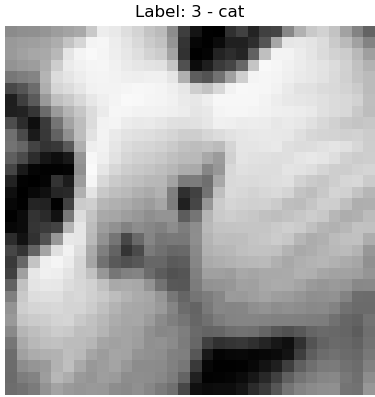
\includegraphics[width=6.0cm]{Definitions/Figure_1.png}}%
\hspace{0.2cm}
\subfloat[\centering Example of the class \textit{truck}]{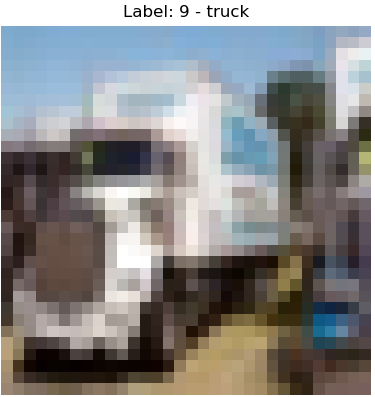
\includegraphics[width=6.0cm]{Definitions/Figure_2.png}}%
\caption{Examples from the dataset used in the project. (\textbf{a}) Image corresponding to the class \textit{cat}. (\textbf{b}) Image corresponding to the class \textit{truck}.\label{fig:exemplo_imagem_dataset}}
\end{figure}

%%%%%%%%%%%%%%%%%%%%%%%%%%%%%%%%%%%%%%%%%%
\section{Development}

The main objective of this work was to compare different machine learning approaches and techniques, assessing their effectiveness in the context of image classification. In particular, CNN's were implemented from scratch, with explicit definition of all layers. Throughout the project, the complexity of the architectures was progressively increased in order to investigate the impact of architectural changes on model performance. Anticipating the risk of \textit{overfitting,} especially in simpler models, various regularization techniques were introduced, such as data augmentation and dropout, aiming to improve generalization. The performance of the developed CNN's was then compared to that of traditional machine learning classifiers, validating the advantages of deep learning methods in this domain. Finally, the implemented CNN's were also compared to state-of-the-art pre-trained models, allowing for a critical analysis of their relative performance and complexity.

\subsection{CNN Architectures}
Convolutional Neural Networks (CNN's) are a class of deep learning models particularly well-suited for image data, due to their ability to extract and learn spatial hierarchies of features directly from the raw pixels. In this project, the implemented CNN architectures incorporate a variety of commonly used layers. \texttt{Conv2d} layers apply a set of learnable filters over local regions of the input image to extract low-level and high-level features. \texttt{ReLU} (Rectified Linear Unit) activation functions introduce non-linearity, allowing the network to model complex patterns. \texttt{BatchNorm2d} layers normalize intermediate activations, accelerating training and improving stability. \texttt{MaxPool2d} layers reduce the spatial dimensions of the feature maps, contributing to translation invariance and helping to control overfitting. After convolutional processing, a \texttt{Flatten} layer reshapes the multi-dimensional feature maps into a 1D vector, which is then passed through one or more \texttt{Linear} (fully connected) layers that perform the final classification. In deeper architectures, \texttt{Dropout} is also employed as a regularization technique that randomly deactivates neurons during training, further mitigating overfitting. These components, when combined, form the basis of powerful CNN architectures capable of learning from complex visual data~\cite{gfg_cnn_intro}.

The \texttt{SimpleCNN} model was implemented as a lightweight baseline to assess the capabilities of a minimal convolutional architecture. It comprises two convolutional layers with a small number of filters, each followed by \texttt{ReLU} activation and \texttt{MaxPool2d} operations, progressively reducing the spatial resolution while increasing feature abstraction. After the convolutional stages, the output is flattened and passed through two fully connected layers, culminating in a final output layer that maps to the number of target classes. This compact design offers a useful reference point for evaluating the effect of increased model depth and complexity. The full structure is depicted in Figure~\ref{fig:arq_simples}.

In contrast, the \texttt{ComplexCNN} model was implemented to explore a deeper and more regularized architecture. It consists of three convolutional blocks, each containing two convolutional layers with \texttt{BatchNorm2d} and \texttt{ReLU} activations, followed by \texttt{MaxPool2d} layers to downsample the spatial dimensions. The feature extractor is followed by a three-layer fully connected head, with \texttt{Dropout} regularization applied after each hidden layer to mitigate overfitting. The final layer outputs class probabilities for the task at hand. This more complex architecture enables the model to learn hierarchical and abstract features with greater representational power. The full architecture is shown in Figure~\ref{fig:arq_complexa}.


\begin{figure}[H]
\begin{adjustwidth}{-\extralength}{0cm}
\centering
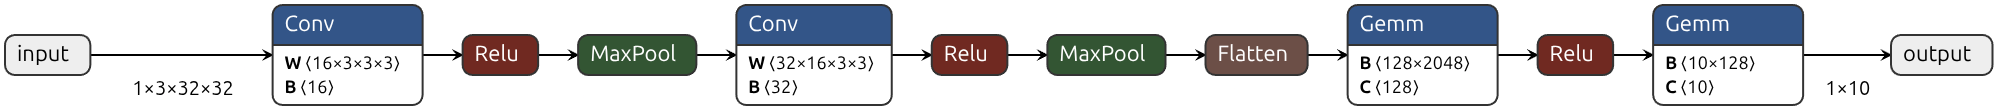
\includegraphics[width=\linewidth]{Definitions/simple_cnn.png}
\end{adjustwidth}
\caption{Simple CNN Architecture \label{fig:arq_simples}}
\end{figure}

\begin{figure}[H]
\begin{adjustwidth}{-\extralength}{0cm}
\centering
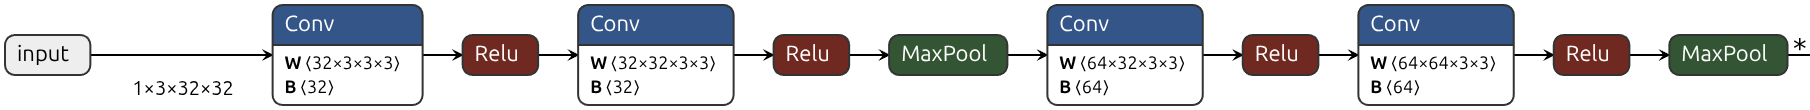
\includegraphics[width=\linewidth]{Definitions/complex_cnn (Copy).png}\\[0.5em]
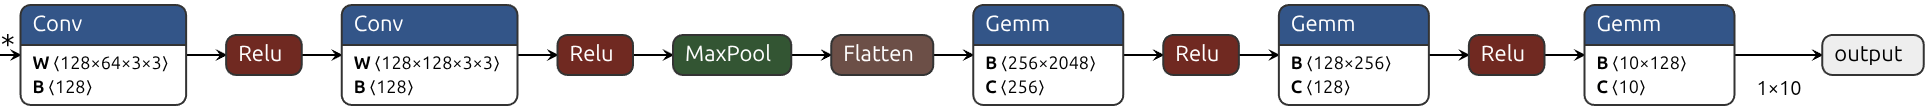
\includegraphics[width=\linewidth]{Definitions/complex_cnn (Copy 2).png}
\end{adjustwidth}
\caption{Complex CNN Architecture \label{fig:arq_complexa}}

\vspace{0.5em}
\noindent{\footnotesize{* The figure is divided into 2 parts}}
\end{figure}

% data augmentation, dropout, batch size, learning rate, número de épocas, funções de ativação, otimizador
\clearpage
\subsection{Training Parameters and Overfitting Mitigation}

The training process was designed to be efficient, reproducible, and consistent across all experiments. The input data, already preprocessed and organized into training, validation, and test sets as described in \autoref{sec:data_processing}, was passed to a custom dataset class implementing the \texttt{torch.utils.data.Dataset} interface. This enabled the integration of real-time transformations during training and evaluation.

During training, the data was loaded in mini-batches of size 32, with \texttt{shuffle} enabled to improve the statistical diversity of each batch. A supervised learning approach was employed, with the model trained for a predefined number of epochs using standard mini-batch gradient descent. The loss function used was \texttt{CrossEntropyLoss}, which is appropriate for multi-class classification tasks. Model parameters were updated using the \texttt{Adam} optimizer, a widely used adaptive optimization algorithm that tries to ensure stable and efficient convergence.

Model performance was evaluated after each epoch using the validation set, allowing for the monitoring of learning progress and early detection of overfitting. Upon completion of training, the model was evaluated on an independent test set to estimate its generalization performance.

\subsubsection{Overfitting and Mitigation Strategies}

Due to the relatively low number of parameters in the implemented convolutional networks, overfitting was expected to be a significant concern. To address this, multiple regularization techniques were incorporated into both the training process and model architecture.

\begin{itemize}
    \item \textbf{Data Augmentation:} To increase the effective size and diversity of the training set, a set of stochastic image transformations was applied at training time. These included random cropping with padding and horizontal flipping. Such augmentations introduce variability and help prevent the model from overfitting to specific training examples~\cite{shorten2019}.

    \item \textbf{Dropout:} Dropout layers were added after certain convolutional and fully connected layers. This technique randomly disables a subset of neurons during training, promoting redundancy in feature representations and reducing co-adaptation.

    \item \textbf{Batch Normalization:} In deeper architectures, batch normalization layers were included after convolutional operations. These layers normalize activations across mini-batches, stabilizing training dynamics and serving as an implicit form of regularization.

    \item \textbf{Weight Decay:} L2 regularization was introduced through the optimizer's weight decay parameter. This penalizes large parameter values and encourages simpler, more generalizable solutions.
\end{itemize}

Together, these mitigation strategies were intended to improve generalization and reduce the performance gap between training and validation phases.




\subsection{Classical Classifiers}
\label{sec:classical_classifiers}


To complement the CNN's developed in this work, a set of classical machine learning classifiers was applied to the deep features extracted from the trained CNN models. This methodology allows for the evaluation of the discriminative capacity of the learned features, independently of the CNN’s final classification layer. Moreover, by providing the same feature representation to multiple classifiers, it becomes possible to assess how much the performance depends on the classifier itself versus the quality of the learned features.

In addition, Principal Component Analysis (PCA) was applied as a dimensionality reduction technique to the extracted features prior to classification. PCA transforms the feature space by projecting it onto a smaller set of orthogonal components that capture the maximum variance in the data. This reduces feature dimensionality and potential noise, which can improve classifier efficiency and generalization.

The classifiers selected represent a variety of modelling assumptions and complexities, enabling a broad evaluation of the feature space.

\subsubsection*{Logistic Regression}

Logistic Regression is a linear classification model that estimates the probability of class membership through the logistic function. Despite its simplicity, it is widely used due to its interpretability and efficiency.

Its inclusion in this context allows to assess whether the feature space produced by the CNN's is linearly separable. If good performance is achieved with this model, it suggests that the CNN was able to learn features that are well-organized in terms of class boundaries.

\subsubsection*{Random Forest}

Random Forest is an ensemble method composed of multiple decision trees trained on random data and feature subsets. It combines the outputs of individual trees to improve generalization and reduce overfitting.

Its use here is justified by its robustness and ability to handle complex, non-linear patterns without requiring extensive hyperparameter tuning. Applying it to deep features enables a comparison with simpler linear models and an evaluation of the richness of the learned representations.

\subsubsection*{K-Nearest Neighbors (KNN)}

KNN is a non-parametric method that classifies a sample based on the majority label among its $K$ nearest training examples. It relies on a distance metric (typically Euclidean) to define proximity in the feature space.

This classifier is particularly well-suited for evaluating the geometric structure of the deep feature space. If CNN's group semantically similar inputs close together, KNN can perform well, despite not involving a learned decision function.

\subsubsection*{Support Vector Machine (SVM)}

The Support Vector Machine constructs decision boundaries that maximize the margin between classes. It supports both linear and non-linear classification through kernel functions.

Due to the high dimensionality of deep features, SVM's are well-suited for this context. Their ability to find robust separating hyperplanes makes them a strong benchmark for evaluating the separability of the learned embeddings, especially with non-linear kernels like RBF (Radial Basis Function).

\subsubsection*{Multi-Layer Perceptron (MLP)}

The MLP is a fully connected feedforward neural network that uses non-linear activation functions to model complex decision boundaries. It is trained using backpropagation and offers more flexibility than traditional classifiers.

Applying an MLP to deep features helps assess whether additional non-linearity beyond the CNN improves performance by capturing patterns that simpler models might miss


\subsection{Pre-trained Models}
\label{sec:pretrained_models}

For the CIFAR-10 dataset, pre-trained convolutional models made available in the \texttt{PyTorch\_CIFAR10} repository by Huy V. Phan~\cite{huyvnphan_pytorch_cifar10} were used. This collection includes well-established architectures such as \texttt{ResNet-18}, \texttt{DenseNet-121}, and \texttt{VGG-19}, all previously trained on the same dataset. These models provide a solid performance reference, leveraging prior training to perform classification directly on the test set.

The use of these pre-trained models proved effective both in saving computational resources and in establishing a robust baseline using state-of-the-art architectures.

% modelo escolhido, vantagens de usar redes pré-treinadas, comparação com os modelos desenvolvidos
%%%%%%%%%%%%%%%%%%%%%%%%%%%%%%%%%%%%%%%%%%
\section{Results and Discussion}
\label{sec:results}

To ensure a fair and consistent comparison between all classifiers and architectures evaluated, the same training configuration was maintained throughout the experiments. All models were trained for \textbf{200 epochs}, with no use of early stopping. This choice ensured that any signs of overfitting could emerge naturally, offering insights into the generalization capacity of each technique.

The optimizer used was Adam, with a learning rate fixed at $0.001$, and mini-batches of size $32$. The loss function adopted was cross-entropy, suitable for multi-class classification tasks. %For models requiring overfitting mitigation, regularization techniques such as dropout, weight decay ($7.5 \times 10^{-4}$), and data augmentation (random cropping and horizontal flipping) were selectively applied.

This uniform setup guarantees that observed differences in performance arise from the models and feature representations themselves, rather than from inconsistencies in the training process.

The results are organized into three main sections corresponding to the simple CNN, the complex CNN, and the pre-trained models. Within each CNN section, results are presented separately for each overfitting correction technique and dataset (CIFAR-10 and CIFAR-100). The pre-trained models are evaluated only on CIFAR-10 due to the availability of pre-trained weights.

\subsection{Simple CNN}

Figure~\ref{fig:cnn_simple_cifar10_no_reg} to Figure~\ref{fig:cnn_simple_cifar100_reg} present the training and validation loss and accuracy curves over 200 epochs for the simple CNN, both without and with overfitting correction techniques, on the CIFAR-10 and CIFAR-100 datasets.

Without regularization (Figures~\ref{fig:cnn_simple_cifar10_no_reg} and \ref{fig:cnn_simple_cifar100_no_reg}), a clear overfitting phenomenon is observed. For CIFAR-10, the training loss quickly drops to near zero, while the validation loss initially decreases but then rises continuously, exceeding 8 by the end of training. The training accuracy reaches 99\%, while validation accuracy peaks around 67\% before declining to about 63\%. 

The effect is even more pronounced on CIFAR-100, where training loss again approaches zero, but validation loss escalates above 22. Training accuracy nearly hits 100\%, while validation accuracy peaks at 33\% before falling to approximately 26\%. This demonstrates the model’s limited generalization capacity, especially with the added complexity of CIFAR-100.

To address overfitting, regularization methods were applied: dropout with a probability of 0.45, weight decay of $7.5 \times 10^{-4}$, and data augmentation via random cropping and horizontal flipping. The impact of these techniques is visible in Figures~\ref{fig:cnn_simple_cifar10_reg} and \ref{fig:cnn_simple_cifar100_reg}. For CIFAR-10, both training and validation losses stabilize around 1.1, with training accuracy at 60\% and validation accuracy fluctuating between 60\% and 67\%, indicating improved generalization.

Similarly, in CIFAR-100, both losses converge near 3.0–3.2, and training and validation accuracies stay close, between 25\% and 32\%, showing that the regularized model avoids memorization and generalizes better despite the dataset's difficulty.


\begin{figure}[H]
\begin{adjustwidth}{-\extralength}{0cm}
\centering
\subfloat[Loss and Accuracy during training and validation on CIFAR-10 without regularization.\label{fig:cnn_simple_cifar10_no_reg}]{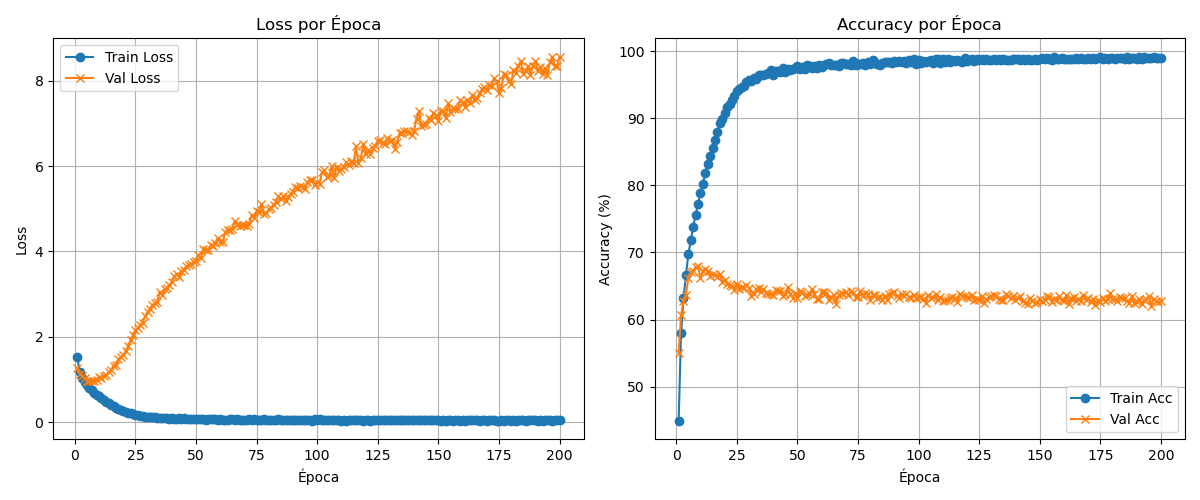
\includegraphics[width=0.72\linewidth]{Definitions/simple_cnn_training_metrics_10_e200.png}}\\[0.5em]
\subfloat[Loss and Accuracy during training and validation on CIFAR-10 with regularization.\label{fig:cnn_simple_cifar10_reg}]{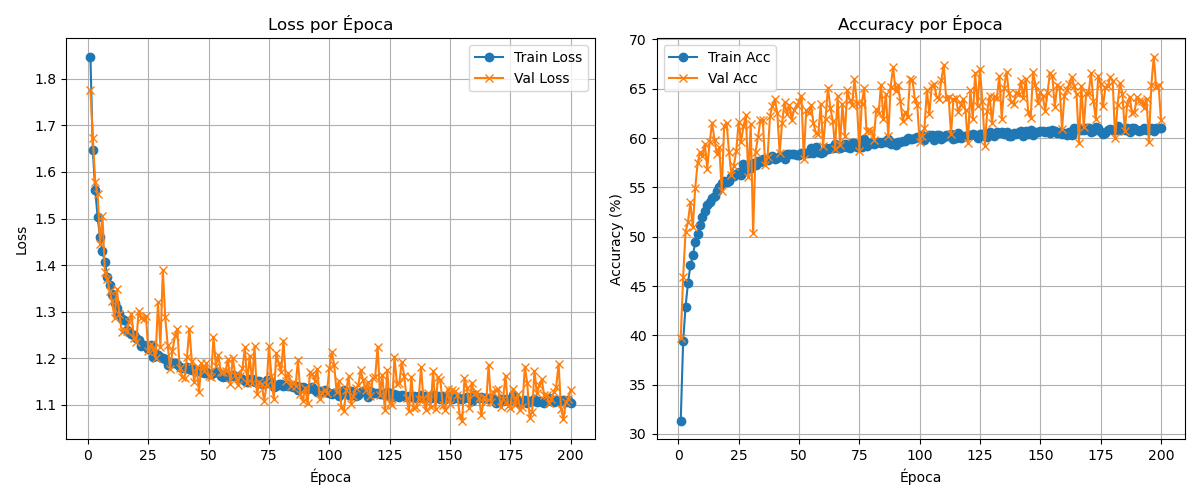
\includegraphics[width=0.72\linewidth]{Definitions/simple_cnn_training_metrics_10_correcao_overfitting_e200.png}}\\[0.5em]
\subfloat[Loss and Accuracy during training and validation on CIFAR-100 without regularization.\label{fig:cnn_simple_cifar100_no_reg}]{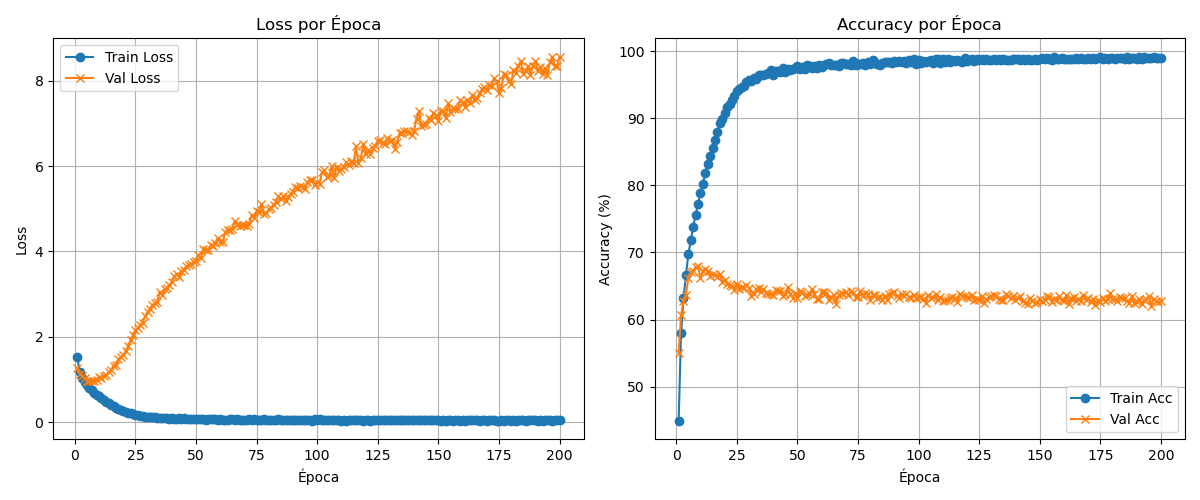
\includegraphics[width=0.72\linewidth]{Definitions/simple_cnn_training_metrics_10_e200.png}}\\[0.5em]
\subfloat[Loss and Accuracy during training and validation on CIFAR-100 with regularization.\label{fig:cnn_simple_cifar100_reg}]{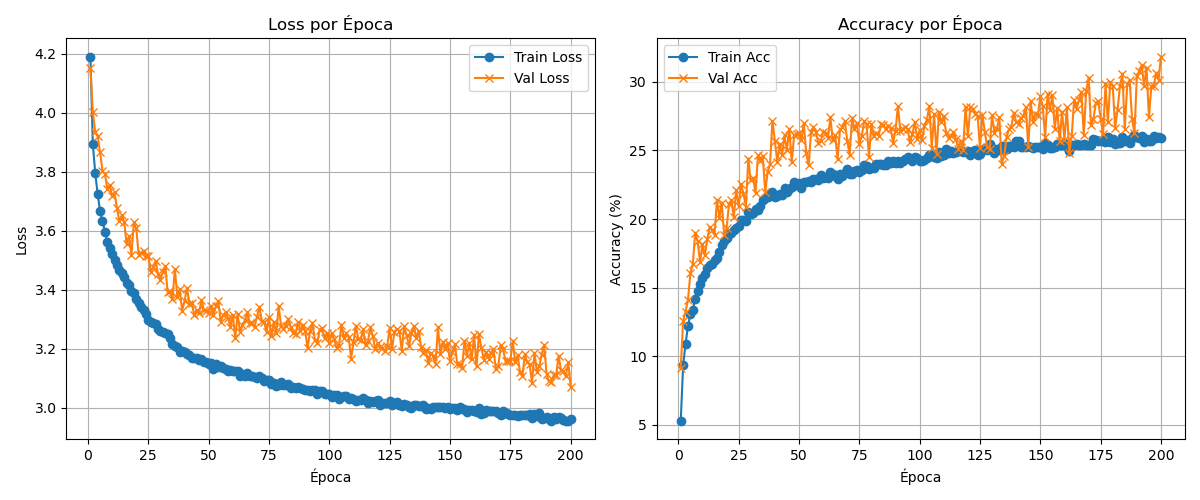
\includegraphics[width=0.72\linewidth]{Definitions/simple_cnn_training_metrics_100_correcao_overfitting_e200.png}}
\end{adjustwidth}
\caption{Training and validation loss and accuracy curves for the simple CNN on CIFAR-10 and CIFAR-100}
\end{figure}


Table~\ref{tab:simple_cnn_summary} summarizes the final training and validation metrics for all four scenarios discussed, providing a concise overview of the model's behavior with and without regularization on each dataset.

Despite the improvements brought by regularization, the overall results remain modest, especially on CIFAR-100. This outcome highlights the necessity for more complex models capable of capturing richer representations and handling higher dataset complexity.

\begin{table}[H]
\caption{Summary of final training and validation results for the simple CNN after 200 epochs.\label{tab:simple_cnn_summary}}
\begin{tabularx}{\textwidth}{lCCCCC}
\toprule
\textbf{Dataset} & \textbf{Regularization} & \textbf{Train Accuracy (\%)} & \textbf{Val Accuracy (\%)} & \textbf{Train Loss} & \textbf{Val Loss} \\
\midrule
CIFAR-10  & No  & $\sim$99 & $\sim$63     & $\sim$0   & $\sim$8.5 \\
CIFAR-10  & Yes & $\sim$60 & 60--67      & $\sim$1.1 & $\sim$1.1 \\
CIFAR-100 & No  & $\sim$99 & $\sim$26     & $\sim$0   & $\sim$22  \\
CIFAR-100 & Yes & $\sim$25 & 25--32      & $\sim$3.0 & $\sim$3.2 \\
\bottomrule
\end{tabularx}
\end{table}

\subsection{Classical Classifiers with Simple CNN}
\label{sec:classificadores_simple_cnn}

The traditional classifiers introduced in \autoref{sec:classical_classifiers} were trained using the features extracted from the simple CNN. Each was evaluated with and without the application of PCA, retaining 95\% of the original variance. This process resulted in the automatic selection of 48 components for CIFAR-10 and 51 for CIFAR-100.

Table~\ref{tab:classifiers_results} summarizes the accuracy and training time for each configuration, while Figures~\ref{fig:classifiers_cifar10_no_pca} to~\ref{fig:classifiers_cifar100_pca} provide a graphical overview of the results.

In the case of CIFAR-10, the highest accuracy (0.46) was obtained without PCA, and PCA reduced training times considerably, particularly for SVM, whose time dropped from 220 to 53 seconds,with only marginal changes in accuracy. The MLP also maintained strong performance while reducing training time by nearly 30\%. 

The CIFAR-100 dataset posed a greater challenge due to its increased class complexity. Accuracy scores were generally lower across all models. Still, both MLP and SVM showed relatively strong results, particularly with PCA applied, reaching 0.20 and 0.22 accuracy, respectively. Notably, PCA not only reduced training times significantly but also led to a substantial improvement in SVM’s performance.

Further insights can be drawn from the confusion matrices for CIFAR-10, included in \autoref{ap:ap1}. The MLP and SVM were notably effective at classifying visually distinct categories such as \textit{ship} (654 correct predictions for MLP), \textit{frog}, and \textit{horse}, but struggled with semantically similar ones like \textit{cat} vs. \textit{dog}, and \textit{automobile} vs \textit{truck}. KNN showed strong bias toward certain classes, such as overpredicting \textit{airplane}, while Logistic Regression demonstrated widespread misclassification in ambiguous categories. Confusion matrices were not included for CIFAR-100 due to the large number of classes, which made visualization and interpretation impractical.


\begin{table}[H]
\caption{Accuracy and training time of traditional classifiers, with and without PCA.\label{tab:classifiers_results}}
\centering
\begin{tabular}{lcccccccc}
\toprule
\multirow{2}{*}{\textbf{Classifier}} & \multicolumn{2}{c}{\textbf{CIFAR-10}} & \multicolumn{2}{c}{\textbf{CIFAR-10 + PCA}} & \multicolumn{2}{c}{\textbf{CIFAR-100}} & \multicolumn{2}{c}{\textbf{CIFAR-100 + PCA}} \\
\cmidrule(lr){2-3} \cmidrule(lr){4-5} \cmidrule(lr){6-7} \cmidrule(lr){8-9}
 & \textbf{Acc.} & \textbf{Time} & \textbf{Acc.} & \textbf{Time} & \textbf{Acc.} & \textbf{Time} & \textbf{Acc.} & \textbf{Time} \\
\midrule
Logistic Regression & 0.37 & 2 & 0.34 & 1 & 0.10 & 2 & 0.11 & 2 \\
Random Forest       & 0.40 & 26 & 0.38 & 24 & 0.16 & 58 & 0.16 & 77 \\
KNN                 & 0.34 & 0 & 0.32 & 0 & 0.13 & 0 & 0.15 & 0 \\
MLP                 & 0.46 & 60 & 0.43 & 42 & 0.19 & 102 & 0.20 & 98 \\
SVM                 & 0.44 & 220 & 0.45 & 53 & 0.16 & 104 & 0.22 & 58 \\
\bottomrule
\end{tabular}
\vspace{0.5em}

\noindent\footnotesize{* Accuracy rounded to two decimal places; training time in seconds.}
\end{table}

\begin{figure}[H]
\begin{adjustwidth}{-\extralength}{0cm}
\centering
\subfloat[Accuracy and training time of classifiers on CIFAR-10 without PCA.\label{fig:classifiers_cifar10_no_pca}]{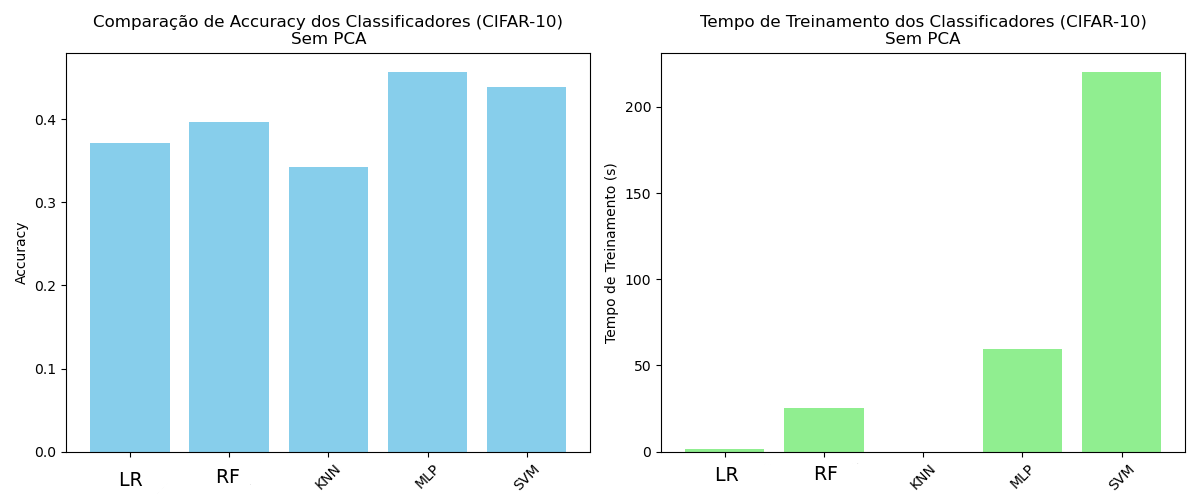
\includegraphics[width=0.72\linewidth]{Definitions/cnn_simples_cifar10_classifiers_comparison_sem_pca.png}}\\[0.5em]
\subfloat[Accuracy and training time of classifiers on CIFAR-10 with PCA.\label{fig:classifiers_cifar10_pca}]{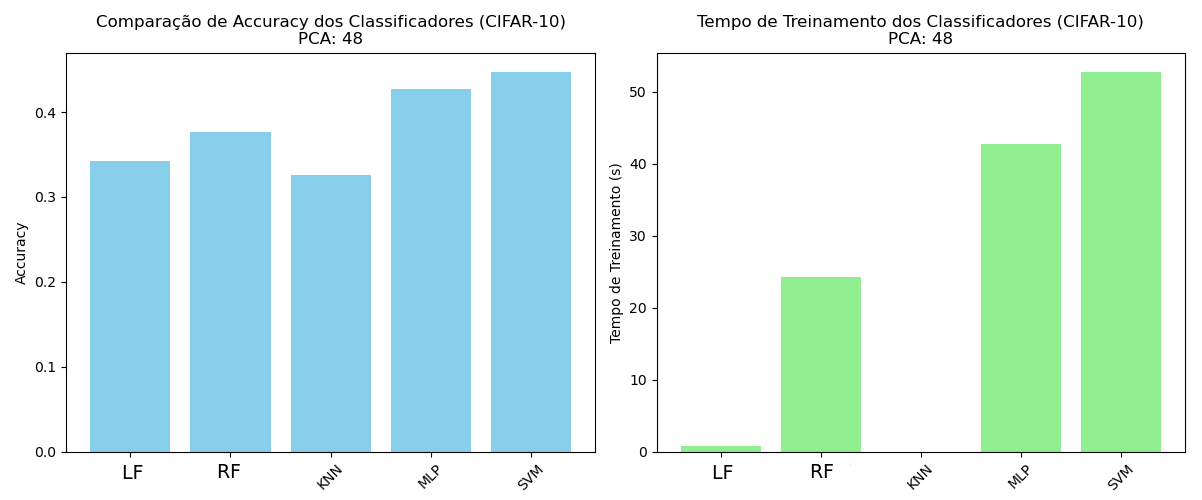
\includegraphics[width=0.72\linewidth]{Definitions/cnn_simples_cifar10_classifiers_comparison_pca48.png}}\\[0.5em]
\subfloat[Accuracy and training time of classifiers on CIFAR-100 without PCA.\label{fig:classifiers_cifar100_no_pca}]{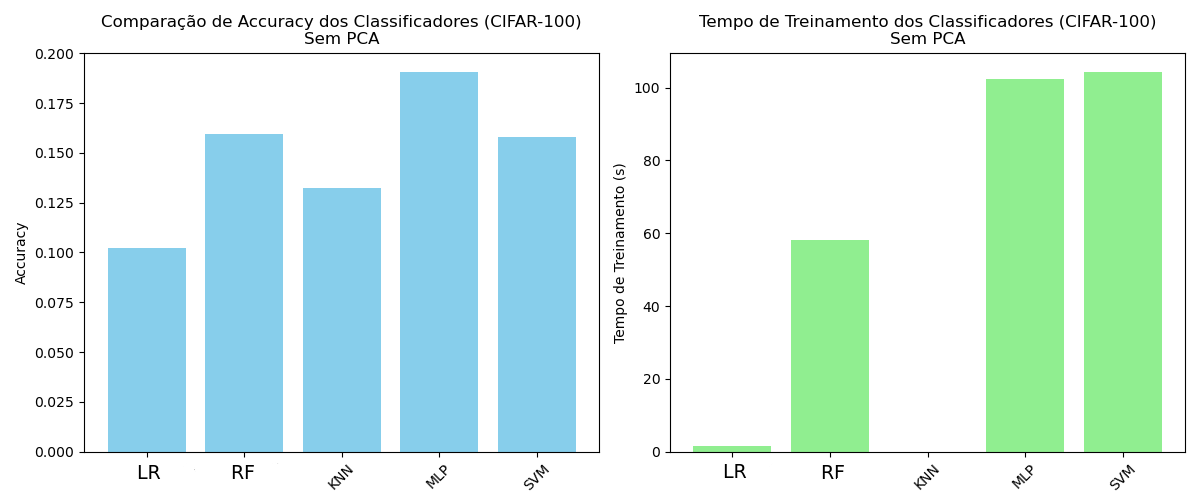
\includegraphics[width=0.72\linewidth]{Definitions/cnn_simples_cifar100_classifiers_comparison_sem_pca.png}}\\[0.5em]
\subfloat[Accuracy and training time of classifiers on CIFAR-100 with PCA.\label{fig:classifiers_cifar100_pca}]{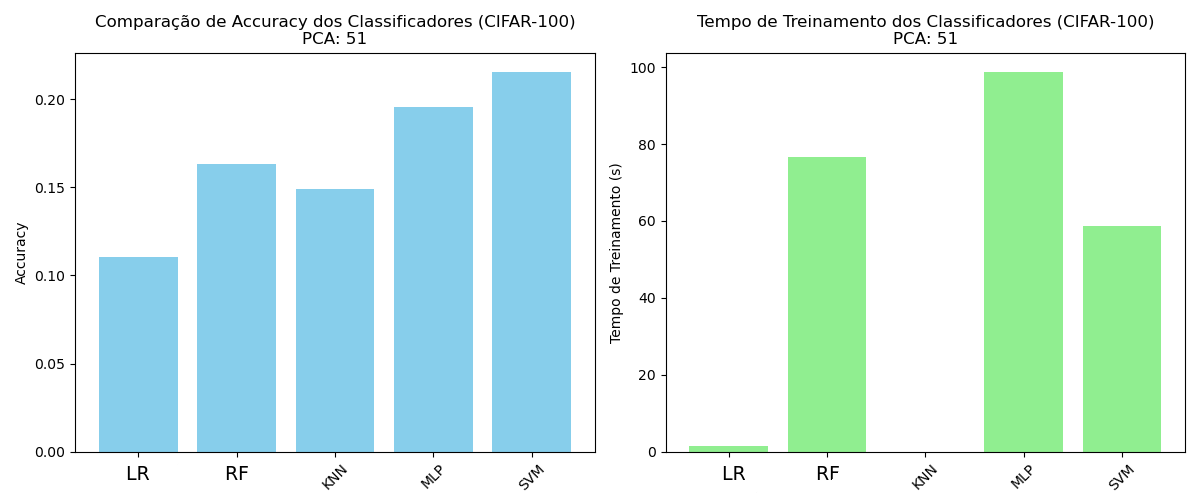
\includegraphics[width=0.72\linewidth]{Definitions/cnn_simples_cifar100_classifiers_comparison_pca51.png}}
\end{adjustwidth}
\caption{Accuracy and training time of classifiers using CNN features, with and without PCA}
\end{figure}

Overall, the results indicate that the most complex classifiers are better equipped to leverage the high-level representations extracted by the CNN, while PCA proves to be a valuable strategy for reducing computational cost with minimal impact on predictive performance.


\subsection{Complex CNN}

To improve upon the results obtained with the simple CNN, a more complex convolutional neural network architecture was designed by adding additional convolutional and fully connected layers. The rationale behind increasing the model depth was to enable the network to capture richer and more abstract feature representations, potentially leading to better performance on the challenging CIFAR-10 and CIFAR-100 datasets.  
The training methodology remained consistent with the previous experiments.

The performance was monitored through the evolution of training and validation loss and accuracy, and the final metrics are summarized to provide a clear comparison between different configurations.

Table~\autoref{tab:complex_cnn_summary} presents the final training and validation results for the complex CNN across CIFAR-10 and CIFAR-100 datasets, with and without overfitting correction techniques. These values were derived from the loss and accuracy curves shown in Figures~\ref{fig:cnn_complex_cifar10_no_reg} to \ref{fig:cnn_complex_cifar100_reg}.

For CIFAR-10 without regularization (Figure~\ref{fig:cnn_complex_cifar10_no_reg}), the training accuracy reached approximately 100\%, with a training loss near zero. The validation accuracy was about 82\%, while the validation loss remained around 1.8. This suggests the model effectively learned the training data and generalized reasonably well to the validation set, although some overfitting may be present given the gap between training and validation loss.

In contrast, when applying overfitting correction on CIFAR-10 (Figure~\ref{fig:cnn_complex_cifar10_reg}), training accuracy dropped to around 75\% with a corresponding training loss near 0.7. The validation accuracy was slightly lower, approximately 80\%, with a validation loss also around 0.7, indicating improved generalization and reduced overfitting effects.

For CIFAR-100 without regularization (Figure~\ref{fig:cnn_complex_cifar100_no_reg}), the model achieved about 80\% training accuracy with training loss near 0.75, but validation accuracy was only around 40\%, with validation loss exceeding 5. This large gap between training and validation metrics indicates pronounced overfitting.

When overfitting correction techniques were applied on CIFAR-100 (Figure~\ref{fig:cnn_complex_cifar100_reg}), the model showed substantially lower training performance, with approximately 32\% training accuracy and a high training loss near 2.5. The validation accuracy remained low at about 36\%, and validation loss ranged between 2.5 and 3.0, reflecting the difficulty of the dataset and the strong regularization limiting model capacity.

These results highlight the trade-offs between model complexity, overfitting correction, and dataset difficulty, illustrating that regularization can improve generalization at the expense of training accuracy, especially on more complex datasets.

\begin{table}[H]
\caption{Summary of final training and validation results for the complex CNN after 200 epochs.\label{tab:complex_cnn_summary}}
\centering
\begin{tabularx}{\textwidth}{lCCCCC}
\toprule
\textbf{Dataset} & \textbf{Regularization} & \textbf{Train Accuracy (\%)} & \textbf{Val Accuracy (\%)} & \textbf{Train Loss} & \textbf{Val Loss} \\
\midrule
CIFAR-10  & No  & $\sim$100 & $\sim$82  & $\sim$0.0 & $\sim$1.8 \\
CIFAR-10  & Yes & $\sim$75  & $\sim$80  & $\sim$0.7 & $\sim$0.7 \\
CIFAR-100 & No  & $\sim$80  & $\sim$40  & $\sim$0.75& $>$5 \\
CIFAR-100 & Yes & $\sim$32  & $\sim$36  & $\sim$2.5 & 2.5--3.0 \\
\bottomrule
\end{tabularx}
\end{table}

\begin{figure}[H]
\begin{adjustwidth}{-\extralength}{0cm}
\centering
\subfloat[Loss and Accuracy during training and validation on CIFAR-10 without regularization.\label{fig:cnn_complex_cifar10_no_reg}]{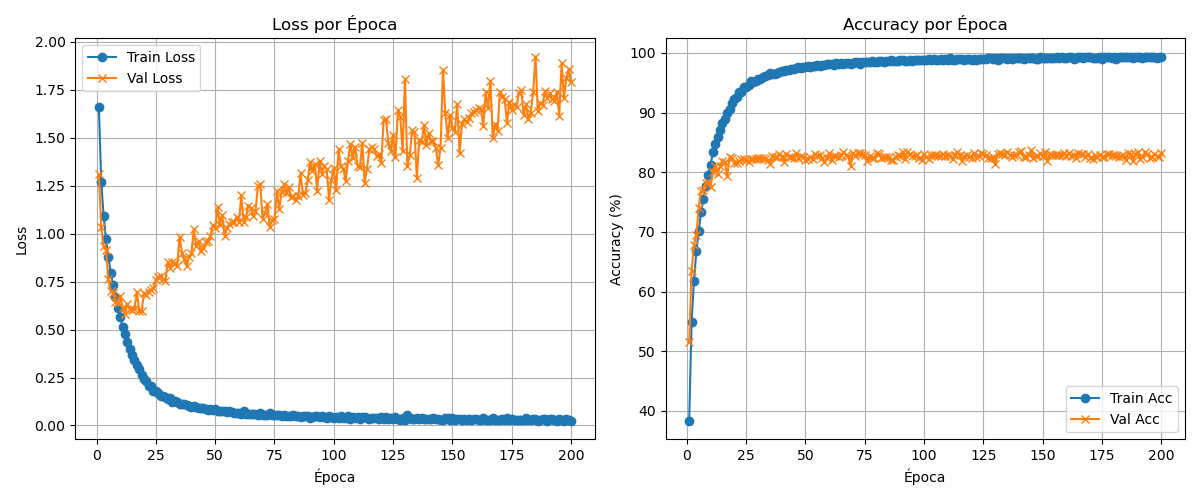
\includegraphics[width=0.72\linewidth]{Definitions/complex_cnn_training_metrics_10_e200.png}}\\[0.5em]
\subfloat[Loss and Accuracy during training and validation on CIFAR-10 with regularization.\label{fig:cnn_complex_cifar100_no_reg}]{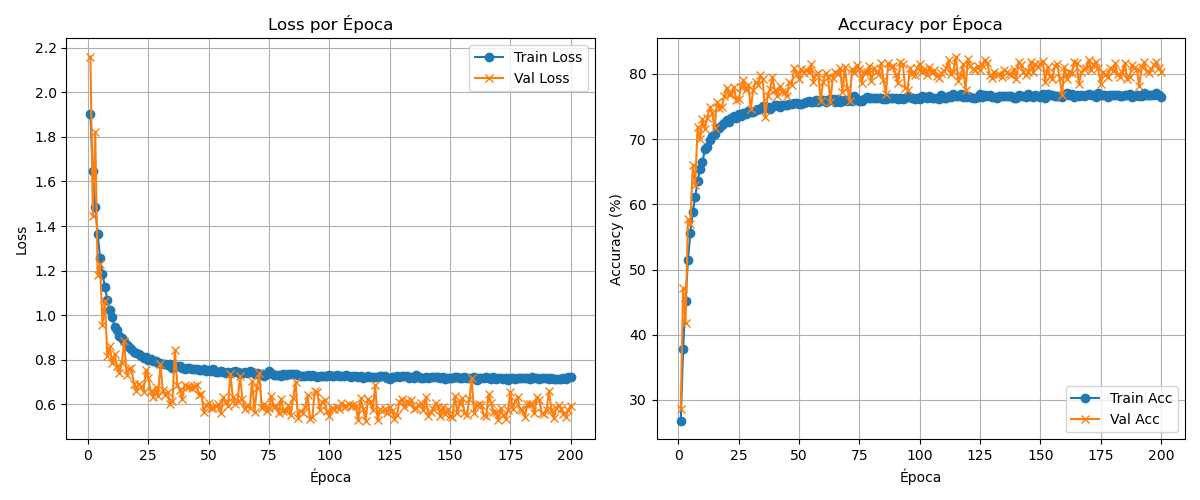
\includegraphics[width=0.72\linewidth]{Definitions/complex_cnn_training_metrics_10_correcao_overfitting_e200.png}}\\[0.5em]
\subfloat[Loss and Accuracy during training and validation on CIFAR-100 without regularization.\label{fig:cnn_complex_cifar10_reg}]{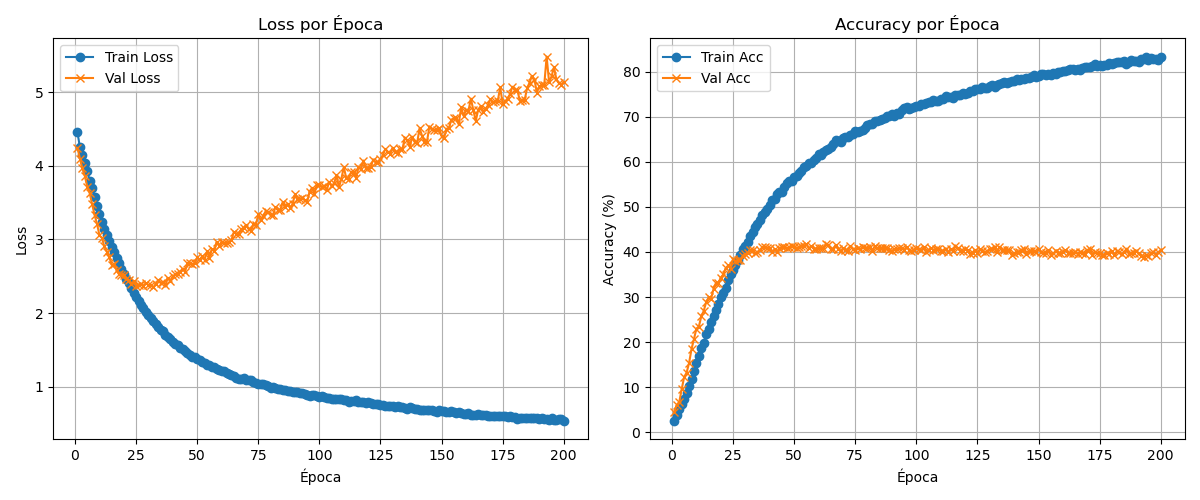
\includegraphics[width=0.72\linewidth]{Definitions/complex_cnn_training_metrics_100_e200.png}}\\[0.5em]
\subfloat[Loss and Accuracy during training and validation on CIFAR-100 with regularization.\label{fig:cnn_complex_cifar100_reg}]{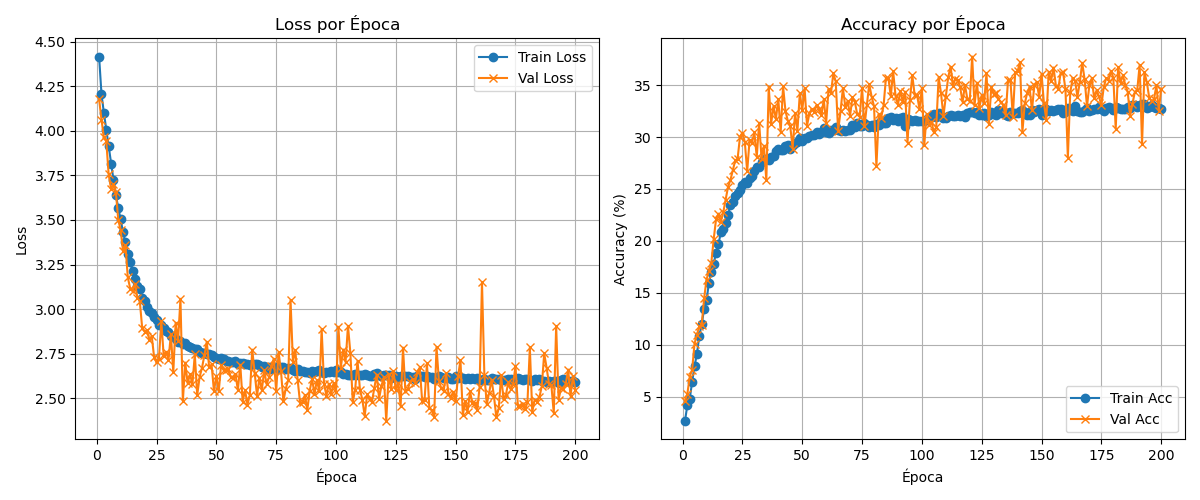
\includegraphics[width=0.72\linewidth]{Definitions/complex_cnn_training_metrics_100_correcao_overfitting_e200.png}}
\end{adjustwidth}
\caption{Training and validation loss and accuracy curves for the simple CNN on CIFAR-10 and CIFAR-100}
\end{figure}
\clearpage

\subsection{Classical Classifiers with Complex CNN}
\label{sec:classical_classifiers_2}

Following the analysis conducted using the simple CNN, the same set of traditional classifiers introduced in \autoref{sec:classical_classifiers} was applied to the features extracted from the more complex CNN. As before, the classifiers were evaluated both with and without the application of PCA, retaining 95\% of the original variance. This resulted in 54 components for CIFAR-10 and 65 for CIFAR-100.

Table~\ref{tab:classifiers_results_complex} summarizes the accuracy and training time for each classifier, and Figures~\ref{fig:classifiers_cifar10_no_pca_complex} to~\ref{fig:classifiers_cifar100_pca_complex} illustrate these results graphically.

On CIFAR-10, the complex CNN provided higher-quality features, leading to improved performance across all classifiers. SVM and MLP were the most effective, reaching accuracies of 0.79 and 0.78 respectively. The application of PCA significantly reduced training time, particularly for SVM (from 64 to 32 seconds), without compromising performance.

A more detailed analysis of class-wise performance can be found in the confusion matrices provided in \autoref{ap:ap2}. As with the simple CNN, classifiers such as MLP and SVM showed high accuracy in visually distinctive categories like \textit{airplane}, \textit{ship}, and \textit{truck}, but struggled with visually or semantically similar categories, especially \textit{cat} vs. \textit{dog}, and \textit{automobile} vs. \textit{truck}. Logistic Regression and KNN exhibited more confusion, particularly in ambiguous categories.

For CIFAR-100, results remained lower overall due to the increased class complexity. SVM and MLP continued to outperform the other methods, achieving accuracies of 0.39 and 0.35 respectively with PCA. Once again, PCA proved effective in reducing computational cost, especially for SVM.

Confusion matrices were not included for CIFAR-100 due to the large number of classes, which made visualization and interpretation impractical.


\begin{table}[H]
\caption{Accuracy and training time of traditional classifiers using features from the complex CNN, for CIFAR-10 and CIFAR-100, with and without PCA.\label{tab:classifiers_results_complex}}
\centering
\begin{tabular}{lcccccccc}
\toprule
\multirow{2}{*}{\textbf{Classifier}} & \multicolumn{2}{c}{\textbf{CIFAR-10}} & \multicolumn{2}{c}{\textbf{CIFAR-10 + PCA}} & \multicolumn{2}{c}{\textbf{CIFAR-100}} & \multicolumn{2}{c}{\textbf{CIFAR-100 + PCA}} \\
\cmidrule(lr){2-3} \cmidrule(lr){4-5} \cmidrule(lr){6-7} \cmidrule(lr){8-9}
 & \textbf{Acc.} & \textbf{Time} & \textbf{Acc.} & \textbf{Time} & \textbf{Acc.} & \textbf{Time} & \textbf{Acc.} & \textbf{Time} \\
\midrule
Logistic Regression & 0.76 & 1 & 0.75 & 1 & 0.29 & 2 & 0.29 & 2 \\
Random Forest       & 0.76 & 26 & 0.75 & 33 & 0.30 & 64 & 0.29 & 84 \\
KNN                 & 0.76 & 0 & 0.75 & 0 & 0.28 & 0 & 0.28 & 0 \\
MLP                 & 0.78 & 68 & 0.78 & 54 & 0.36 & 105 & 0.35 & 87 \\
SVM                 & 0.79 & 64 & 0.79 & 32 & 0.37 & 58 & 0.39 & 48 \\
\bottomrule
\end{tabular}
\vspace{0.5em}

\noindent\footnotesize{* Accuracy rounded to two decimal places; training time in seconds.}
\end{table}

Overall, the results suggest that the additional depth and capacity of the complex CNN contribute to higher-quality feature representations, which are more effectively leveraged by advanced classifiers such as SVM and MLP. PCA remains a valuable tool for reducing computational cost without significantly impacting classification performance.

\begin{figure}[H]
\begin{adjustwidth}{-\extralength}{0cm}
\centering
\subfloat[Accuracy and training time of classifiers on CIFAR-10 without PCA.\label{fig:classifiers_cifar10_no_pca_complex}]{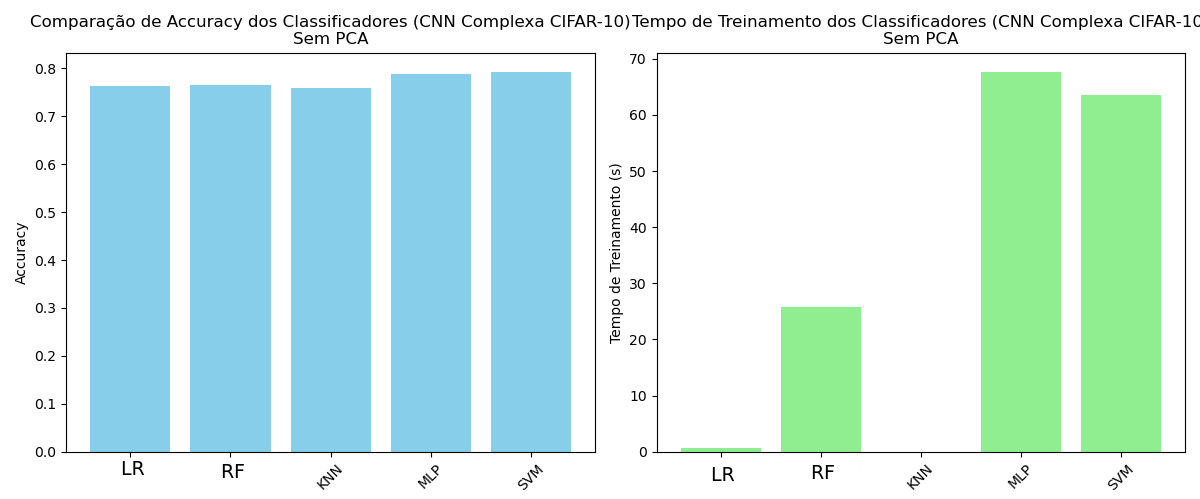
\includegraphics[width=0.72\linewidth]{Definitions/cnn_complexa_cifar10_classifiers_comparison_sem_pca.png}}\\[0.5em]
\subfloat[Accuracy and training time of classifiers on CIFAR-10 with PCA.\label{fig:classifiers_cifar10_pca_complex}]{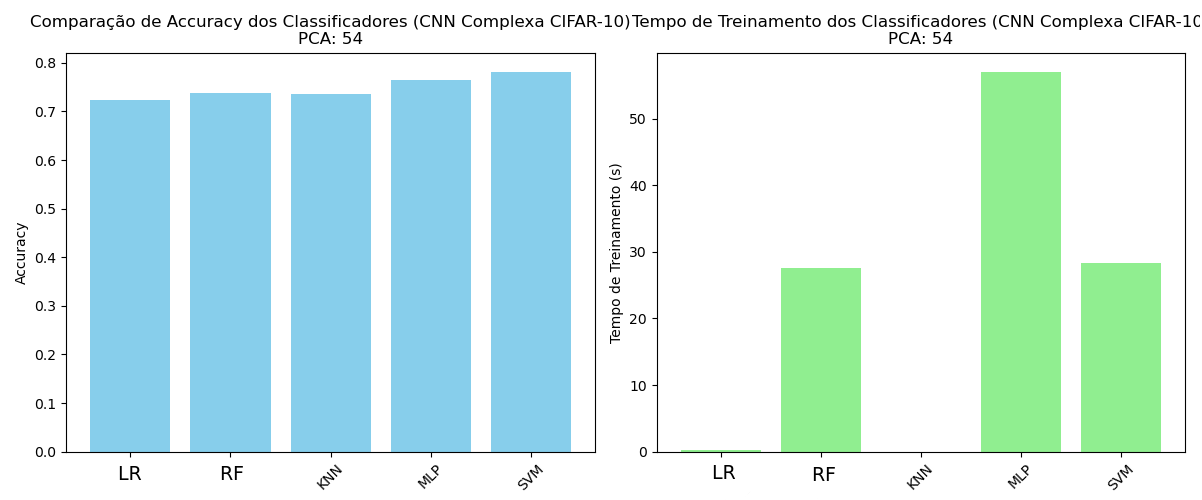
\includegraphics[width=0.72\linewidth]{Definitions/cnn_complexa_cifar10_classifiers_comparison_pca54.png}}\\[0.5em]
\subfloat[Accuracy and training time of classifiers on CIFAR-100 without PCA.\label{fig:classifiers_cifar100_no_pca_complex}]{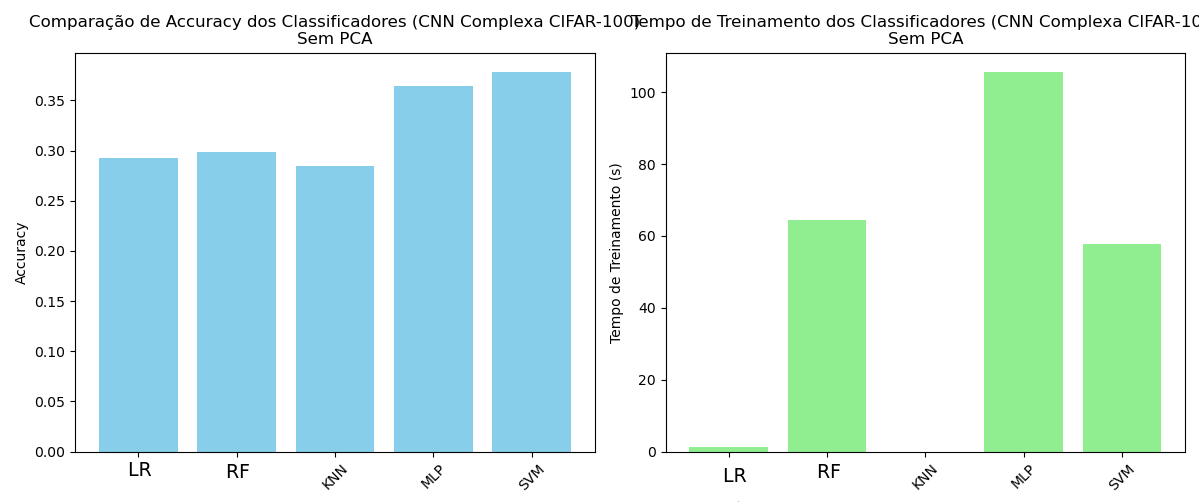
\includegraphics[width=0.72\linewidth]{Definitions/cnn_complexa_cifar100_classifiers_comparison_sem_pca.png}}\\[0.5em]
\subfloat[Accuracy and training time of classifiers on CIFAR-100 with PCA.\label{fig:classifiers_cifar100_pca_complex}]{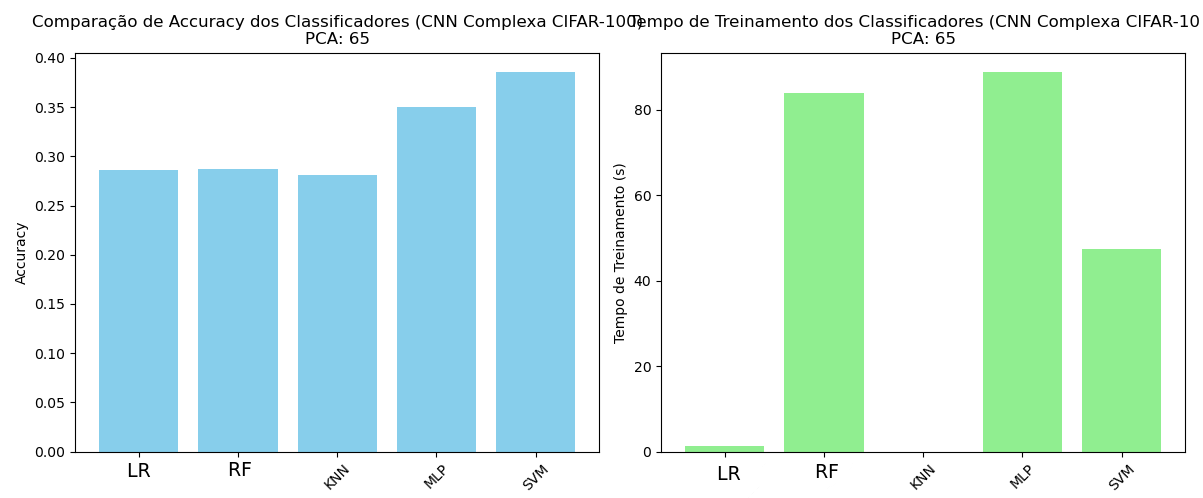
\includegraphics[width=0.72\linewidth]{Definitions/cnn_complexa_cifar100_classifiers_comparison_pca65.png}}
\end{adjustwidth}
\caption{Accuracy and training time of classifiers using CNN features, with and without PCA.}
\end{figure}


\clearpage

\subsection{Pre-trained Models}
\label{sec:pretrained_models_results}

The evaluation of pre-trained models on CIFAR-10 yielded high classification accuracy across all tested architectures. \autoref{tab:pretrained_results} presents the accuracy scores obtained by each model.


\begin{table}[H]
\caption{Accuracy of pre-trained models on CIFAR-10.\label{tab:pretrained_results}}
\centering
\begin{tabular}{lc}
\toprule
\textbf{Model} & \textbf{Accuracy} \\
\midrule
ResNet-18     & 93.08\% \\
DenseNet-121  & 94.06\% \\
VGG-19        & 93.35\% \\
\bottomrule
\end{tabular}
\vspace{0.5em}

\noindent\footnotesize{* Accuracy values are reported as percentages.}
\end{table}

\texttt{DenseNet-121} achieved the highest performance, reaching an accuracy of 94.06\%. \texttt{ResNet-18} and \texttt{VGG-19} followed closely, with 93.08\% and 93.35\%, respectively. While the differences are relatively small, they reflect the architectural advantages of more recent models, such as \texttt{DenseNet’s} dense connectivity and feature reuse.

Overall, all models achieved state-of-the-art performance on CIFAR-10, establishing strong baselines for comparison.

\section{Final Discussion}
\label{sec:final_discussion}

The results obtained throughout this work provide a comprehensive perspective on the challenges and limitations inherent to image classification, even when using datasets as established as CIFAR-10 and CIFAR-100. Despite the adoption of best practices in data preprocessing, regularization, and model design, the implemented CNN's did not reach state-of-the-art performance, especially on CIFAR-100, where the highest validation accuracy remained well below the benchmarks reported in the literature. This outcome highlights the substantial complexity of the task: even “basic” datasets like CIFAR-100 present significant obstacles due to their high intra-class variability and the large number of categories, demanding models with greater representational capacity and more sophisticated training strategies.

On CIFAR-10, the results were more encouraging. The simple CNN, when regularized, achieved validation accuracies in the 60–67\% range, while the complex CNN, with appropriate overfitting mitigation, reached approximately 80\%. These values, although distant from the 90\%+ accuracy of pre-trained models, are notable given the relatively modest depth and parameter count of the custom architectures. The observed gap between training and validation performance in the absence of regularization further reinforces the importance of techniques such as data augmentation, dropout, and weight decay in promoting generalization.

The experiments with classical classifiers corroborate the trends described in the state-of-the-art section. When applied directly to deep features extracted from the CNN's, traditional models like Logistic Regression, Random Forest, KNN, SVM, and MLP consistently underperformed relative to the fully connected layers of the neural networks. Their accuracy was particularly limited when using features from the simpler CNN, but improved markedly as the complexity of the feature extractor increased. This demonstrates that the discriminative power of classical classifiers is heavily dependent on the quality of the input representation, a finding that aligns with the broader consensus in the literature.

The application of PCA as a dimensionality reduction technique proved to be a valuable strategy for managing computational resources. In almost all scenarios, PCA significantly reduced training times, especially for computationally intensive models like SVM, without causing a substantial drop in accuracy. In some cases, such as SVM on CIFAR-100, PCA even led to improved performance, likely due to noise reduction and better feature compactness. This suggests that, in practical settings, dimensionality reduction can be leveraged to balance efficiency and predictive power.

Finally, the evaluation of pre-trained models on CIFAR-10 established a clear upper bound for performance, with \texttt{DenseNet-121}, \texttt{ResNet-18}, and \texttt{VGG-19} all achieving accuracies above 93\%. The substantial gap between these results and those obtained with custom CNN's underscores the impact of architectural advances, large-scale training, and hyperparameter optimization in achieving state-of-the-art results.

In summary, this work demonstrates that while deep learning models, especially CNN's, are essential for tackling image classification tasks, achieving top-tier performance requires not only careful model design and regularization, but also access to advanced architectures and extensive computational resources. The experiments reinforce the importance of feature quality for downstream classifiers and highlight PCA as a practical tool for resource management. Above all, the persistent difficulty of CIFAR-100 serves as a reminder that even “basic” benchmarks remain challenging and continue to drive progress in the field.

%%%%%%%%%%%%%%%%%%%%%%%%%%%%%%%%%%%%%%%%%%


%%%%%%%%%%%%%%%%%%%%%%%%%%%%%%%%%%%%%%%%%%
%% optional
%\supplementary{The following supporting information can be downloaded at:  \linksupplementary{s1}, Figure S1: title; Table S1: title; Video S1: title.}

% Only for journal Methods and Protocols:
% If you wish to submit a video article, please do so with any other supplementary material.
% \supplementary{The following supporting information can be downloaded at: \linksupplementary{s1}, Figure S1: title; Table S1: title; Video S1: title. A supporting video article is available at doi: link.}

% Only used for preprtints:
% \supplementary{The following supporting information can be downloaded at the website of this paper posted on \href{https://www.preprints.org/}{Preprints.org}.}

% Only for journal Hardware:
% If you wish to submit a video article, please do so with any other supplementary material.
% \supplementary{The following supporting information can be downloaded at: \linksupplementary{s1}, Figure S1: title; Table S1: title; Video S1: title.\vspace{6pt}\\
%\begin{tabularx}{\textwidth}{lll}
%\toprule
%\textbf{Name} & \textbf{Type} & \textbf{Description} \\
%\midrule
%S1 & Python script (.py) & Script of python source code used in XX \\
%S2 & Text (.txt) & Script of modelling code used to make Figure X \\
%S3 & Text (.txt) & Raw data from experiment X \\
%S4 & Video (.mp4) & Video demonstrating the hardware in use \\
%... & ... & ... \\
%\bottomrule
%\end{tabularx}
%}

%%%%%%%%%%%%%%%%%%%%%%%%%%%%%%%%%%%%%%%%%%
%\authorcontributions{For research articles with several authors, a short paragraph specifying their individual contributions must be provided. The following statements should be used ``Conceptualization, X.X. and Y.Y.; methodology, X.X.; software, X.X.; validation, X.X., Y.Y. and Z.Z.; formal analysis, X.X.; investigation, X.X.; resources, X.X.; data curation, X.X.; writing---original draft preparation, X.X.; writing---review and editing, X.X.; visualization, X.X.; supervision, X.X.; project administration, X.X.; funding acquisition, Y.Y. All authors have read and agreed to the published version of the manuscript.'', please turn to the  \href{http://img.mdpi.org/data/contributor-role-instruction.pdf}{CRediT taxonomy} for the term explanation. Authorship must be limited to those who have contributed substantially to the work~reported.}

%\funding{Please add: ``This research received no external funding'' or ``This research was funded by NAME OF FUNDER grant number XXX.'' and  and ``The APC was funded by XXX''. Check carefully that the details given are accurate and use the standard spelling of funding agency names at \url{https://search.crossref.org/funding}, any errors may affect your future funding.}

%\institutionalreview{In this section, you should add the Institutional Review Board Statement and approval number, if relevant to your study. You might choose to exclude this statement if the study did not require ethical approval. Please note that the Editorial Office might ask you for further information. Please add “The study was conducted in accordance with the Declaration of Helsinki, and approved by the Institutional Review Board (or Ethics Committee) of NAME OF INSTITUTE (protocol code XXX and date of approval).” for studies involving humans. OR “The animal study protocol was approved by the Institutional Review Board (or Ethics Committee) of NAME OF INSTITUTE (protocol code XXX and date of approval).” for studies involving animals. OR “Ethical review and approval were waived for this study due to REASON (please provide a detailed justification).” OR “Not applicable” for studies not involving humans or animals.}

%\informedconsent{Any research article describing a study involving humans should contain this statement. Please add ``Informed consent was obtained from all subjects involved in the study.'' OR ``Patient consent was waived due to REASON (please provide a detailed justification).'' OR ``Not applicable'' for studies not involving humans. You might also choose to exclude this statement if the study did not involve humans.

%Written informed consent for publication must be obtained from participating patients who can be identified (including by the patients themselves). Please state ``Written informed consent has been obtained from the patient(s) to publish this paper'' if applicable.}

%\dataavailability{We encourage all authors of articles published in MDPI journals to share their research data. In this section, please provide details regarding where data supporting reported results can be found, including links to publicly archived datasets analyzed or generated during the study. Where no new data were created, or where data is unavailable due to privacy or ethical restrictions, a statement is still required. Suggested Data Availability Statements are available in section ``MDPI Research Data Policies'' at \url{https://www.mdpi.com/ethics}.} 

% Only for journal Drones
%\durcstatement{Current research is limited to the [please insert a specific academic field, e.g., XXX], which is beneficial [share benefits and/or primary use] and does not pose a threat to public health or national security. Authors acknowledge the dual-use potential of the research involving xxx and confirm that all necessary precautions have been taken to prevent potential misuse. As an ethical responsibility, authors strictly adhere to relevant national and international laws about DURC. Authors advocate for responsible deployment, ethical considerations, regulatory compliance, and transparent reporting to mitigate misuse risks and foster beneficial outcomes.}

% Only for journal Nursing Reports
%\publicinvolvement{Please describe how the public (patients, consumers, carers) were involved in the research. Consider reporting against the GRIPP2 (Guidance for Reporting Involvement of Patients and the Public) checklist. If the public were not involved in any aspect of the research add: ``No public involvement in any aspect of this research''.}
%
%% Only for journal Nursing Reports
%\guidelinesstandards{Please add a statement indicating which reporting guideline was used when drafting the report. For example, ``This manuscript was drafted against the XXX (the full name of reporting guidelines and citation) for XXX (type of research) research''. A complete list of reporting guidelines can be accessed via the equator network: \url{https://www.equator-network.org/}.}
%
%% Only for journal Nursing Reports
%\useofartificialintelligence{Please describe in detail any and all uses of artificial intelligence (AI) or AI-assisted tools used in the preparation of the manuscript. This may include, but is not limited to, language translation, language editing and grammar, or generating text. Alternatively, please state that “AI or AI-assisted tools were not used in drafting any aspect of this manuscript”.}

%\acknowledgments{In this section you can acknowledge any support given which is not covered by the author contribution or funding sections. This may include administrative and technical support, or donations in kind (e.g., materials used for experiments). Where GenAI has been used for purposes such as generating text, data, or graphics, or for study design, data collection, analysis, or interpretation of data, please add “During the preparation of this manuscript/study, the author(s) used [tool name, version information] for the purposes of [description of use]. The authors have reviewed and edited the output and take full responsibility for the content of this publication.”}

%\conflictsofinterest{Declare conflicts of interest or state ``The authors declare no conflicts of interest.'' Authors must identify and declare any personal circumstances or interest that may be perceived as inappropriately influencing the representation or interpretation of reported research results. Any role of the funders in the design of the study; in the collection, analyses or interpretation of data; in the writing of the manuscript; or in the decision to publish the results must be declared in this section. If there is no role, please state ``The funders had no role in the design of the study; in the collection, analyses, or interpretation of data; in the writing of the manuscript; or in the decision to publish the results''.} 

%%%%%%%%%%%%%%%%%%%%%%%%%%%%%%%%%%%%%%%%%%
%% Optional

%% Only for journal Encyclopedia
%\entrylink{The Link to this entry published on the encyclopedia platform.}

\abbreviations{Abbreviations}{
The following abbreviations are used in this manuscript:
\\

\noindent 
\begin{tabular}{@{}ll}
RGB & Red Green Blue \\
CNN & Convolutional Neural Network \\
CVPR & Conference on Computer Vision and Pattern Recognition \\
SVM & Support Vector Machine \\
KNN & K-Nearest Neighbors \\
MLP & Multi-Layer Perceptron \\
PCA & Principal Component Analysis \\
GPU & Graphics Processing Unit \\
ReLU & Rectified Linear Unit \\
L2 & Euclidean Norm (used in regularization) \\
RBF & Radial Basis Function \\
\end{tabular}
}

\clearpage
%%%%%%%%%%%%%%%%%%%%%%%%%%%%%%%%%%%%%%%%%%
%% Optional
\appendixtitles{yes} % Leave argument "no" if all appendix headings stay EMPTY (then no dot is printed after "Appendix A"). If the appendix sections contain a heading then change the argument to "yes".
\appendixstart
\appendix
\section[\appendixname~\thesection]{Confusion Matrices of Classifiers (Simple CNN)}
\label{ap:ap1}

This appendix presents the confusion matrices obtained for the classical classifiers evaluated on the CIFAR-10 dataset without PCA, using features extracted from the simple CNN. These matrices provide a detailed view of the classification performance across individual classes, highlighting which categories are more frequently confused and which are better distinguished by each model. This additional information complements the quantitative analysis presented in \autoref{sec:classificadores_simple_cnn}, offering a more nuanced understanding of each classifier’s behaviour.

\begin{figure}[H]
\begin{adjustwidth}{-\extralength}{0cm} % tira a margem à esquerda para “expandir” a largura da figura
\centering
\subfloat[Confusion matrix of Logistic Regression.\label{fig:confmat_lr}]{
  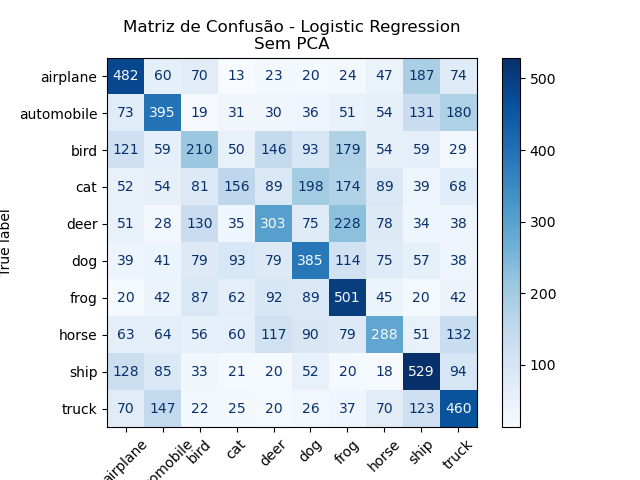
\includegraphics[width=0.39\linewidth]{Definitions/cnn_simples_confusion_matrix_logistic_regression_sem_pca_cifar10.png}
}\hfill
\subfloat[Confusion matrix of Random Forest.\label{fig:confmat_rf}]{
  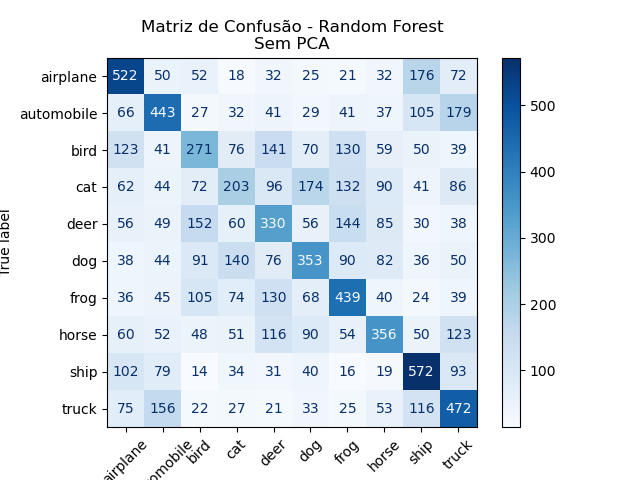
\includegraphics[width=0.39\linewidth]{Definitions/cnn_simples_confusion_matrix_random_forest_sem_pca_cifar10.png}
}\\[1em]
\subfloat[Confusion matrix of KNN.\label{fig:confmat_knn}]{
  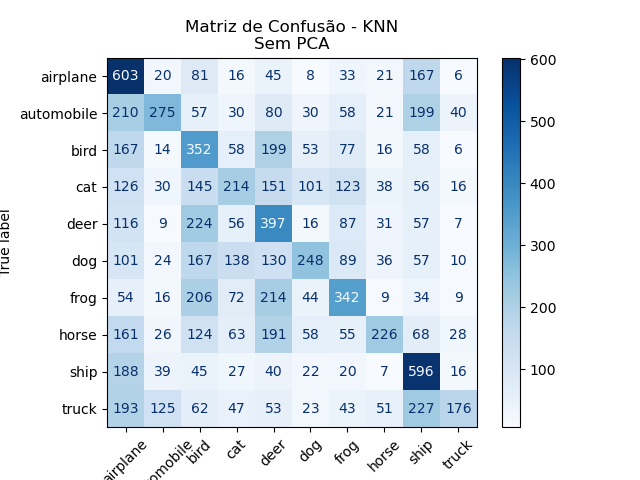
\includegraphics[width=0.39\linewidth]{Definitions/cnn_simples_confusion_matrix_knn_sem_pca_cifar10.png}
}\hfill
\subfloat[Confusion matrix of MLP.\label{fig:confmat_mlp}]{
  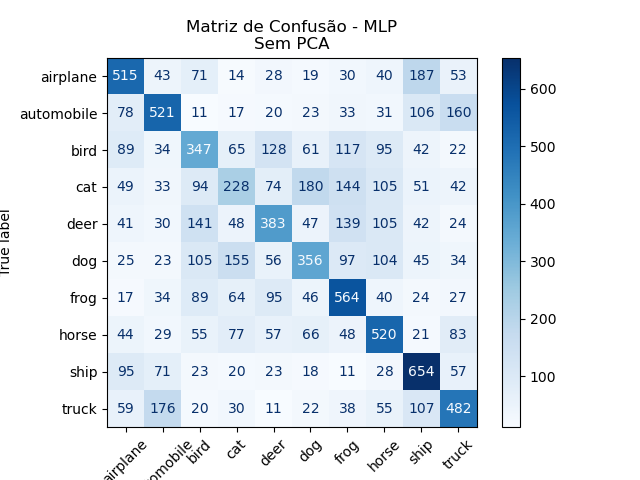
\includegraphics[width=0.39\linewidth]{Definitions/cnn_simples_confusion_matrix_mlp_sem_pca_cifar10.png}
}\\[1em]
\subfloat[Confusion matrix of SVM.\label{fig:confmat_svm}]{
  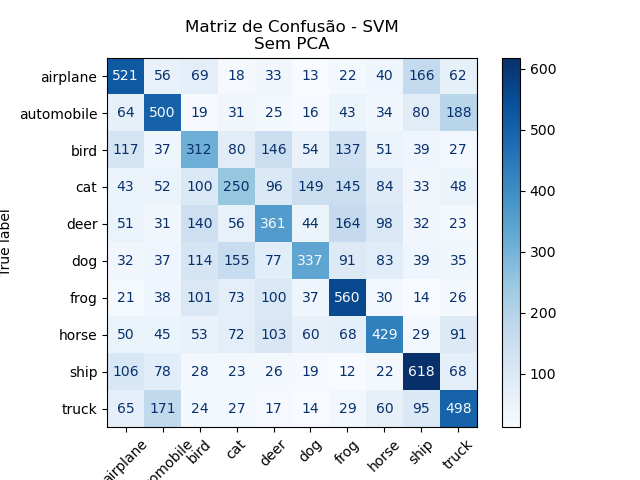
\includegraphics[width=0.39\linewidth]{Definitions/cnn_simples_confusion_matrix_svm_sem_pca_cifar10.png}
}
\end{adjustwidth}
\caption{Confusion matrices for classical classifiers on CIFAR-10 without PCA.\label{fig:confmats_cifar10_sem_pca2}}
\end{figure}



\clearpage
\section[\appendixname~\thesection]{Confusion Matrices of Classifiers (Complex CNN)}
\label{ap:ap2}

This appendix presents the confusion matrices obtained for the classical classifiers evaluated on the CIFAR-10 dataset without PCA, using features extracted from the complex CNN. These matrices provide a detailed view of the classification performance across individual classes, highlighting which categories are more frequently confused and which are better distinguished by each model. This additional information complements the quantitative analysis presented in \autoref{sec:classical_classifiers_2}, offering a more nuanced understanding of each classifier’s behaviour.

\begin{figure}[H]
\begin{adjustwidth}{-\extralength}{0cm} % tira a margem à esquerda para “expandir” a largura da figura
\centering
\subfloat[Confusion matrix of Logistic Regression.\label{fig:confmat_lr2}]{
  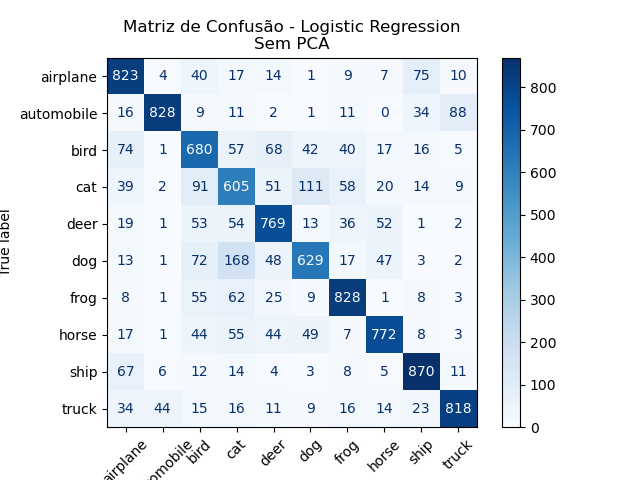
\includegraphics[width=0.39\linewidth]{Definitions/cnn_complexa_confusion_matrix_logistic_regression_sem_pca_cifar10.png}
}\hfill
\subfloat[Confusion matrix of Random Forest.\label{fig:confmat_rf2}]{
  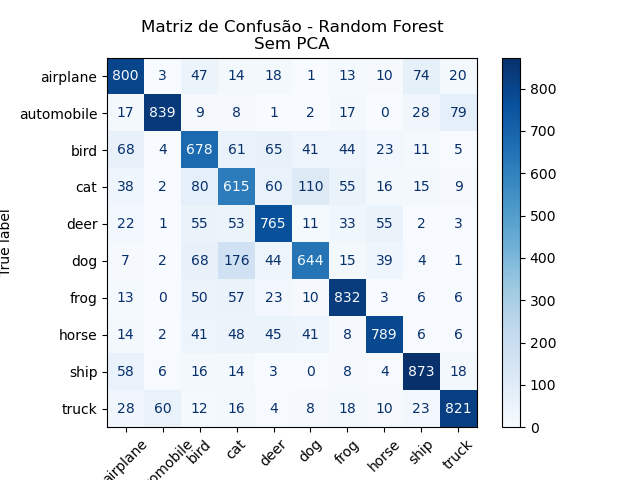
\includegraphics[width=0.39\linewidth]{Definitions/cnn_complexa_confusion_matrix_random_forest_sem_pca_cifar10.png}
}\\[1em]
\subfloat[Confusion matrix of KNN.\label{fig:confmat_knn2}]{
  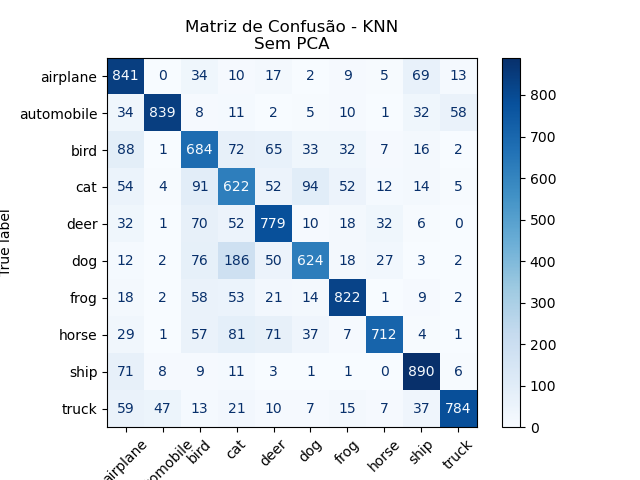
\includegraphics[width=0.39\linewidth]{Definitions/cnn_complexa_confusion_matrix_knn_sem_pca_cifar10.png}
}\hfill
\subfloat[Confusion matrix of MLP.\label{fig:confmat_mlp2}]{
  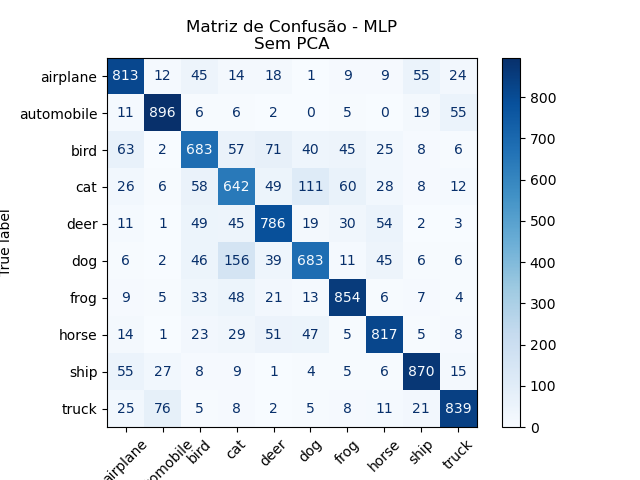
\includegraphics[width=0.39\linewidth]{Definitions/cnn_complexa_confusion_matrix_mlp_sem_pca_cifar10.png}
}\\[1em]
\subfloat[Confusion matrix of SVM.\label{fig:confmat_svm2}]{
  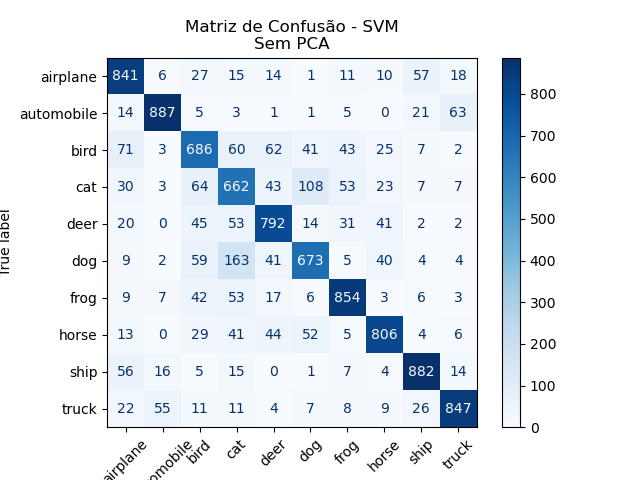
\includegraphics[width=0.39\linewidth]{Definitions/cnn_complexa_confusion_matrix_svm_sem_pca_cifar10.png}
}
\end{adjustwidth}
\caption{Confusion matrices for classical classifiers on CIFAR-10 without PCA.\label{fig:confmats_cifar10_sem_pca}}
\end{figure}

%%%%%%%%%%%%%%%%%%%%%%%%%%%%%%%%%%%%%%%%%%
%\isPreprints{} % If the paper is ``preprints'', please uncomment this parenthesis.
%\printendnotes[custom] % Un-comment to print a list of endnotes

\reftitle{References}

% Please provide either the correct journal abbreviation (e.g. according to the “List of Title Word Abbreviations” http://www.issn.org/services/online-services/access-to-the-ltwa/) or the full name of the journal.
% Citations and References in Supplementary files are permitted provided that they also appear in the reference list here. 

%=====================================
% References, variant A: external bibliography
%=====================================
% \bibliography{your_external_BibTeX_file}

%=====================================
% References, variant B: internal bibliography
%=====================================
% ACS format
\isAPAandChicago{}{%
\begin{thebibliography}{999}
%\begin{thebibliography}{9}

\bibitem{huyvnphan_pytorch_cifar10}
Huy V. Phan. \textit{PyTorch models trained on CIFAR-10 dataset}. GitHub repository. Available at: \url{https://github.com/huyvnphan/PyTorch_CIFAR10}. Accessed: May 31, 2025.

\bibitem{krizhevsky2009}
A.~Krizhevsky and G.~Hinton, \emph{Learning multiple layers of features from tiny images}, University of Toronto, Technical Report, 2009. Available: \url{http://www.cs.toronto.edu/~kriz/learning-features-2009-TR.pdf}

\bibitem{torralba2008}
A.~Torralba, R.~Fergus, and W.~T.~Freeman, “80 million tiny images: A large dataset for nonparametric object and scene recognition,” \emph{IEEE Transactions on Pattern Analysis and Machine Intelligence}, vol.~30, no.~11, pp.~1958–1970, 2008. doi: \url{10.1109/TPAMI.2008.128}

\bibitem{hunter2007}
J.~D.~Hunter, ``Matplotlib: A 2D graphics environment,'' \emph{Computing in Science \& Engineering}, vol.~9, no.~3, pp.~90--95, 2007. doi: \url{10.1109/MCSE.2007.55}

\bibitem{pedregosa2011}
F.~Pedregosa \emph{et al.}, ``Scikit-learn: Machine Learning in Python,'' \emph{Journal of Machine Learning Research}, vol.~12, pp.~2825--2830, 2011.

\bibitem{paszke2019}
A.~Paszke \emph{et al.}, ``PyTorch: An Imperative Style, High-Performance Deep Learning Library,'' in \emph{Advances in Neural Information Processing Systems}, vol.~32, 2019.

\bibitem{marcel2010}
S.~Marcel and Y.~Rodriguez, ``Torchvision the Machine Vision Package of Torch,'' in \emph{Proceedings of the ACM International Conference on Multimedia}, 2010.

\bibitem{pickle}
Python Software Foundation, ``\texttt{pickle} --- Python object serialization,'' \url{https://docs.python.org/3/library/pickle.html}, accessed May 2025.

\bibitem{pytorchdocs}
PyTorch Contributors. \textit{PyTorch Documentation: Data Loading and Processing Tutorial}. Available at: \url{https://pytorch.org/tutorials/beginner/data_loading_tutorial.html} (Accessed: 2025).

\bibitem{tresnet}
Ridnik, T., Lawen, H., Noy, A., Ben-Baruch, E., Sharir, G., and Friedman, I. \textit{TResNet: High Performance GPU-Dedicated Architecture}. Available at: \url{https://github.com/Alibaba-MIIL/TResNet} (Accessed: 2025).

\bibitem{gfg_cnn_intro}
S.~Singh, ``Introduction to Convolutional Neural Networks,'' \emph{GeeksforGeeks}, 2023. [Online]. Available: \url{https://www.geeksforgeeks.org/introduction-convolution-neural-network/}

\bibitem{efficientnet}
Tan, M. and Le, Q. V. \textit{EfficientNet: Rethinking Model Scaling for Convolutional Neural Networks}. arXiv preprint arXiv:1905.11946. Available at: \url{https://arxiv.org/abs/1905.11946} (Accessed: 2025).

\bibitem{resnet}
He, K., Zhang, X., Ren, S., and Sun, J. \textit{Deep Residual Learning for Image Recognition}. In: Proceedings of the IEEE Conference on Computer Vision and Pattern Recognition (CVPR), 2016.

\bibitem{wideresnet}
Zagoruyko, S. and Komodakis, N. \textit{Wide Residual Networks}. arXiv preprint arXiv:1605.07146. Available at: \url{https://arxiv.org/abs/1605.07146} (Accessed: 2025).

\bibitem{densenet}
Huang, G., Liu, Z., Van Der Maaten, L., and Weinberger, K. Q. \textit{Densely Connected Convolutional Networks}. In: Proceedings of the IEEE Conference on Computer Vision and Pattern Recognition (CVPR), 2017.

\bibitem{researchgate1}
ResearchGate. \textit{CNN vs SVM on CIFAR-10 Classification}. Available at: \url{https://www.researchgate.net/publication/335264157} (Accessed: 2025).

\bibitem{shorten2019}
C.~Shorten and T.~M.~Khoshgoftaar, “A survey on image data augmentation for deep learning,” \emph{Journal of Big Data}, vol.~6, no.~1, pp.~1–48, 2019. doi: \url{10.1186/s40537-019-0197-0}

\end{thebibliography}
}

% If authors have biography, please use the format below
%\section*{Short Biography of Authors}
%\bio
%{\raisebox{-0.35cm}{\includegraphics[width=3.5cm,height=5.3cm,clip,keepaspectratio]{Definitions/author1.pdf}}}
%{\textbf{Firstname Lastname} Biography of first author}
%
%\bio
%{\raisebox{-0.35cm}{\includegraphics[width=3.5cm,height=5.3cm,clip,keepaspectratio]{Definitions/author2.jpg}}}
%{\textbf{Firstname Lastname} Biography of second author}

% For the MDPI journals use author-date citation, please follow the formatting guidelines on http://www.mdpi.com/authors/references
% To cite two works by the same author: \citeauthor{ref-journal-1a} (\citeyear{ref-journal-1a}, \citeyear{ref-journal-1b}). This produces: Whittaker (1967, 1975)
% To cite two works by the same author with specific pages: \citeauthor{ref-journal-3a} (\citeyear{ref-journal-3a}, p. 328; \citeyear{ref-journal-3b}, p.475). This produces: Wong (1999, p. 328; 2000, p. 475)

%%%%%%%%%%%%%%%%%%%%%%%%%%%%%%%%%%%%%%%%%%
%% for journal Sci
%\reviewreports{\\
%Reviewer 1 comments and authors’ response\\
%Reviewer 2 comments and authors’ response\\
%Reviewer 3 comments and authors’ response
%}
%%%%%%%%%%%%%%%%%%%%%%%%%%%%%%%%%%%%%%%%%%
%\PublishersNote{}
%\isPreprints{} % If the paper is ``preprints'', please uncomment this parenthesis.
\end{document}

